\documentclass[12pt]{article}
%\usepackage[utf8]{inputenc}
%\documentclass[UTF8]{ctexart}
%\usepackage[UTF8, heading = false, scheme = plain]{ctex}
\usepackage{geometry}
%geometry{a4paper,scale=0.9}
\geometry{a4paper,left=1cm,right=1cm,top=1cm,bottom=2cm}
\usepackage{amsfonts}
\usepackage{color}
\usepackage{url}
%\usepackage{biblatex}
\usepackage{amsmath}
\usepackage{amssymb}
\usepackage{latexsym}
\usepackage[ruled,lined]{algorithm2e}
\usepackage{pythonhighlight}
\usepackage{cite}
%\addbibresource{ref.bib}
%\bibliography{ref.bib}
\usepackage{caption}
\usepackage{graphicx, subfig}
\usepackage{float}
%\usepackage[fontset=ubuntu]{ctex}
%\usepackage{fontspec}
\usepackage{xeCJK}
%\usepackage[colorlinks,
%anchorcolor=black,
%citecolor=black]{hyperref}
%\setmainfont{SimSun}
\usepackage[section]{placeins}
\usepackage{enumitem}
\usepackage{framed}
\usepackage[framemethod=TikZ]{mdframed}
\usepackage{indentfirst}
\usepackage{setspace}%使用间距宏包
\linespread{1.5}
%\title{预备知识}
%\author{leolinuxer }
%\date{June 2020}


\title{GBDT、XGBoost、LightGBM\cite{Zhihu_Understanding_GBDT}\cite{Zhihu_Understanding_GBDT_2}}
%\author{leolinuxer }
%\date{June 2020}

\begin{document}
%\setlength{\parindent}{0pt}
\maketitle
\tableofcontents

\section{GBDT}
\subsection{背景如何在不改变原有模型的结构上提升模型的拟合能力}

假设现在你有样本集$(x_1,y_1),(x_2,y_2),\cdots,(x_n,y_n)$,然后你用一个模型,如$F(x)$去拟合这些数据,使得这批样本的平方损失函数(即$\frac{1}{2}\sum_0^n(y_i-F(x_i))^2$)最小。但是你发现虽然模型的拟合效果很好,但仍然有一些差距,比如预测值 $F(x_1)=0.8$,而真实值$y_1=0.9$,另外你不允许更改原来模型$F(x)$的参数,那么你有什么办法进一步来提高模型的拟合能力呢。

既然不能更改原来模型的参数,那么意味着必须在原来模型的基础之上做改善,那么直观的做法就是建立一个新的模型 $f(x)$ 来拟合 $F(x)$ 未完全拟合真实样本的残差,即$y-F(x)$。所以新模型需要拟合的样本集就变成了:$(x_1,y_1-F(x_1)),(x_2,y_2-F(x_2)),\cdots,(x_n,y_n-F(x_n))$

\subsection{基于残差的 GBDT}
在第一部分,$y_i-F(x_i)$被称为残差,这一部分也就是前一模型($F(x_i)$)未能完全拟合的部分,所以交给新的模型来完成。

我们知道 GBDT 的全称是Gradient Boosting Decision Tree,其中 Gradient 被称为梯度,更一般的理解,可以认为是一阶导,那么这里的残差与梯度是什么关系呢。在第一部分,我们提到了一个叫做平方损失函数的东西,具体形式可以写成$\frac{1}{2}\sum_0^n(y_i-F(x_i))^2$,熟悉其他算法的原理应该知道,\textbf{这个损失函数主要针对回归类型的问题,分类则是用熵值类的损失函数}。具体到平方损失函数的式子,你可能已经发现它的一阶导其实就是残差的形式,所以基于残差的 GBDT 是一种特殊的 GBDT 模型,它的损失函数是平方损失函数,常用来处理回归类的问题。具体形式可以如下表示:

\textbf{损失函数:} $L(y,F(x)) =\frac{1}{2}(y_i-F(x))^2 $

\textbf{我们希望最小化:} $J=\frac{1}{2}\sum_0^n(y_i-F(x_i))^2$

损失函数的一阶导:
$$\frac{\partial J}{\partial F(x_i)} = \frac{\partial \sum_iL(y_i,F(x_i))}{\partial F(x_i)}=\frac{\partial L(y_i,F(x_i))}{\partial F(x_i)} = F(x_i)-y_i$$

正好残差就是负梯度:
$$
y_i-F(x_i) = -\frac{\partial J}{\partial F(x_i)} 
$$

\subsection{为什么基于残差的 GBDT 不是一个好的选择}

基于残差的gbdt在解决回归问题上不算是一个好的选择,一个比较明显的缺点就是对异常值过于敏感。所以一般回归类的损失函数会用绝对损失或者 Huber 损失函数来代替平方损失函数:

\begin{itemize}[itemindent=2em]
    \item 绝对值 (absolute loss): 
    $L(y,F) = |y-F|$
    
    \item Huber损失 (huber loss): 
    $L(y,F) = \begin{cases}
\frac{1}{2}(y-F)^2 & |y-F| <= \delta\\
\delta|y-f(x)|-\frac{1}{2}\delta^2 & |y-F| > \delta\\
\end{cases}$
\end{itemize}

\subsection{Boosting的加法模型}
如前面所述,GBDT 模型可以认为是是由 k 个基模型组成的一个加法运算式:
$$
\hat{y_i} = \sum_{k=1}^K{f_k(x_i)}, f_k \in F
$$

其中 F 是指所有基模型组成的函数空间。

那么一般化的损失函数是预测值 $\hat{y}$ 与 真实值 $y$ 之间的关系,如我们前面的平方损失函数,那么对于n个样本来说,则可以写成:
$$
L = \sum_{i=1}^n{l(y_i,\hat{y_i})}
$$

更一般的,我们知道一个好的模型,在偏差和方差上有一个较好的平衡,而算法的损失函数正是代表了模型的偏差面,最小化损失函数,就相当于最小化模型的偏差,但同时我们也需要兼顾模型的方差,所以目标函数还包括抑制模型复杂度的正则项,因此目标函数可以写成:
$$
Obj = \sum_{i=1}^n{l(y_i,\hat{y_i})} + \sum_{k=1}^{K}\Omega(f_k)
$$

其中 $\Omega(f_k)$ 代表了基模型的复杂度,若基模型是树模型,则树的深度、叶子节点数等指标可以反应树的复杂程度。

对于Boosting来说,它采用的是前向优化算法,即从前往后,逐渐建立基模型来优化逼近目标函数,具体过程如下:

\begin{eqnarray*}
 && \hat{y}_i^0 = 0 \\
 && \hat{y}_i^1 = f_1(x_i)= \hat{y}_i^0 + f_1(x_i)\\
 && \hat{y}_i^2 = f_1(x_i) + f_2(x_i) = \hat{y}_i^1 + f_2(x_i) \\
 && \cdots \\
 && \hat{y}_i^t = \sum_{k=1}^tf_k(x_i) = \hat{y}_i^{t-1} + f_t(x_i)
\end{eqnarray*}

那么,在每一步,如何学习一个新的模型呢,答案的关键还是在于 GBDT 的目标函数上,即新模型的加入总是以优化目标函数为目的的。

我们以第t步的模型拟合为例,在这一步,模型对第 $i$ 个样本 $x_i$ 的预测为:
$$
\hat{y}_i^t = \hat{y}_i^{t-1} + f_t(x_i)
$$

其中 $f_t(x_i)$ 就是我们这次需要加入的新模型,即需要拟合的模型,此时,目标函数就可以写成:
$$
Obj^{(t)} = \sum_{i=1}^n{l(y_i,\hat{y}_i^t)} + \sum_{i=i}^{t}\Omega(f_i) = \sum_{i=1}^n{l(y_i,\hat{y}_i^{t-1} + f_t(x_i))} + \Omega(f_t) + constant
$$

即此时最优化目标函数,就相当于求得了$f_t(x_i)$

\subsection{什么是 GBDT 的目标函数}
根据泰勒公式推导二阶导(GBDT是一阶导,xgboost是二阶导):
$$
f(x+\Delta x) \approx f(x) + f'(x)\Delta x + \frac{1}{2}f''(x)\Delta x^2
$$

\textbf{建立 $Obj$ 表达式和二阶泰勒展开的对应关系}:

\begin{itemize}[itemindent=2em]
    \item $l(y_i,\hat{y}_i^{t-1})$ 对应泰勒公式中的$f(x)$
    
    \item $\hat{y}_i^{t-1}$ 对应泰勒公式中的 $x$
    
    \item $f_t(x_i)$ 对应泰勒公式中的 $\Delta x$
    
    \item $l(y_i,\hat{y}_i^{t-1} + f_t(x_i))$ 对应泰勒公式中的 $f(x+\Delta x)$
\end{itemize}

那么,对 $l(y_i,\hat{y}_i^{t-1} + f_t(x_i))$ 进行二阶泰勒展开后,可以得到:
$$
Obj^{(t)} = \sum_{i=1}^n[l(y_i,\hat{y}_i^{t-1}) + g_if_t(x_i) + \frac{1}{2}h_if_t^2(x_i)] + \Omega (f_t) + constant
$$

其中,
\begin{itemize}[itemindent=2em]
    \item $g_i$ 是损失函数的一阶导,对应泰勒公式中的 $f'(x)$
    
    \item $h_i$ 是损失函数的二阶导,对应泰勒公式中的 $f''(x)$
\end{itemize}

注意是对 $\hat{y}_i^{t-1}$ 求导。以 平方损失函数为例:
\begin{eqnarray*}
    && \sum_{i=1}^n(y_i - (\hat{y}_i^{t-1}+f_t(x_i)))^2 \\
    && g_i = \partial{\frac{(\hat{y}_i^{t-1} - y_i)^2}{\hat{y}^{t-1}}} = 2(\hat{y}^{t-1} - y_i) \\
    && h_i = \partial ^2{\frac{(\hat{y}_i^{t-1} - y_i)^2}{\hat{y}^{t-1}}} = 2
\end{eqnarray*}

由于在第t步$\hat{y}_i^{t-1}$是是一个已知的值,所以 $l(y_i,\hat{y}_i^{t-1})$ 是一个常数,其对函数优化不会产生影响,因此,可以将 $Obj^{(t)}$ 改写为
$$
Obj^{(t)} \approx \sum_{i=1}^n[g_if_t(x_i) + \frac{1}{2}h_if_t^2(x_i)] + \Omega (f_t) + constant
$$

所以我么只要求出每一步损失函数的一阶和二阶导的值(由于前一步的 $\hat{y}_i^{t-1}$ 是已知的,所以这两个值就是常数)代入上述等式,然后最优化目标函数,就可以得到每一步的$f(x)$ ,最后根据加法模型得到一个整体模型。

\subsection{未完待续:如何生成一颗新的树}
\section{XGBoost(非常详细)\cite{Detail_Of_XGBoost_GBDT}\cite{Decision_Tree_XGBoost_LightGBM}}
\subsection{从“目标函数”开始,生成一棵树}
\subsubsection{XGB目标函数}
XGBoost的目标函数由\textbf{训练损失}和\textbf{正则化}项两部分组成,目标函数定义如下:
\begin{figure}[H]
    \centering
    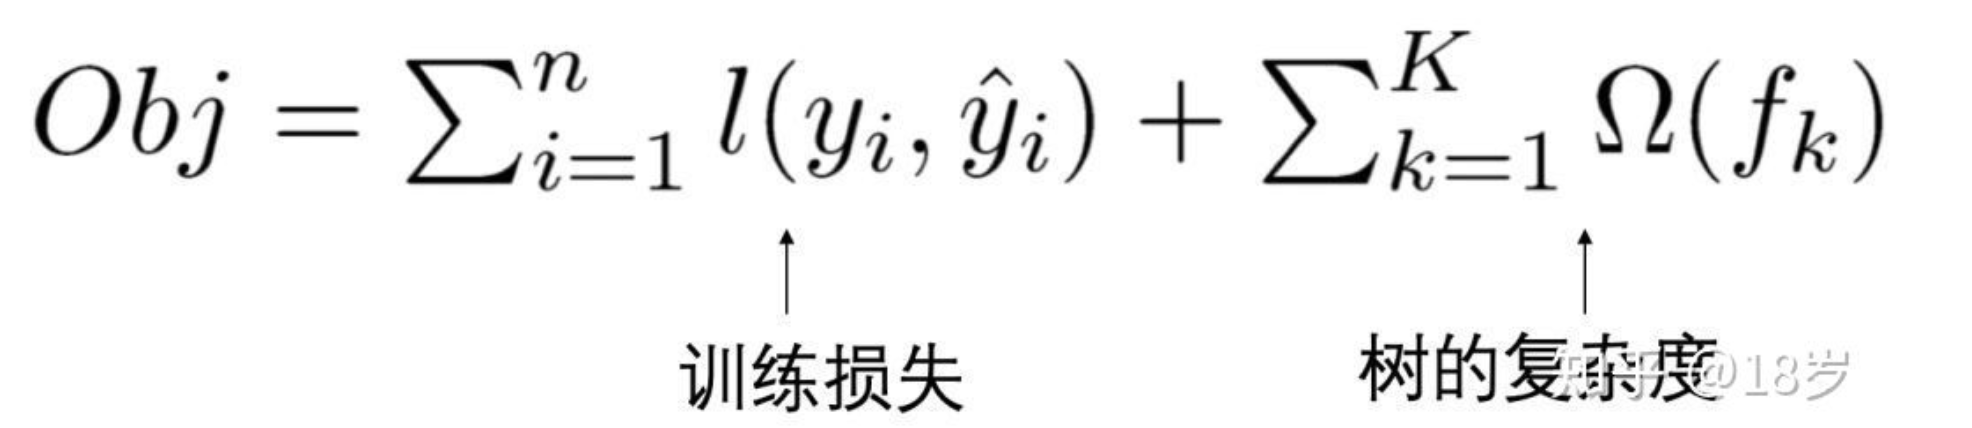
\includegraphics[width=.8\textwidth]{fig/XGBoost_Eq_Objective.png}
\end{figure}

变量解释
\begin{itemize}
\setlength{\itemsep}{0pt}
\setlength{\parsep}{0pt}
\setlength{\parskip}{0pt}
    \item $l$ 代表损失函数,常见的损失函数有:
    $$
    \text{平方损失函数:} \qquad\qquad l(y_i, \hat{y}_i) = (y_i - \hat{y}_i)^2
    $$
    $$
    \text{逻辑回归损失函数:} \qquad l(y_i, \hat{y}_i) = y_i \ln (1+e^{-\hat{y}_i}) + (1-y_i)\ln (1+e^{\hat{y}_i})
    $$
    \item $\hat{y}_i$是第 $i$个样本 $x_i$的预测值。由于XGBoost是一个加法模型,因此,预测得分是每棵树打分的累加之和:
    \begin{figure}[H]
    \centering
    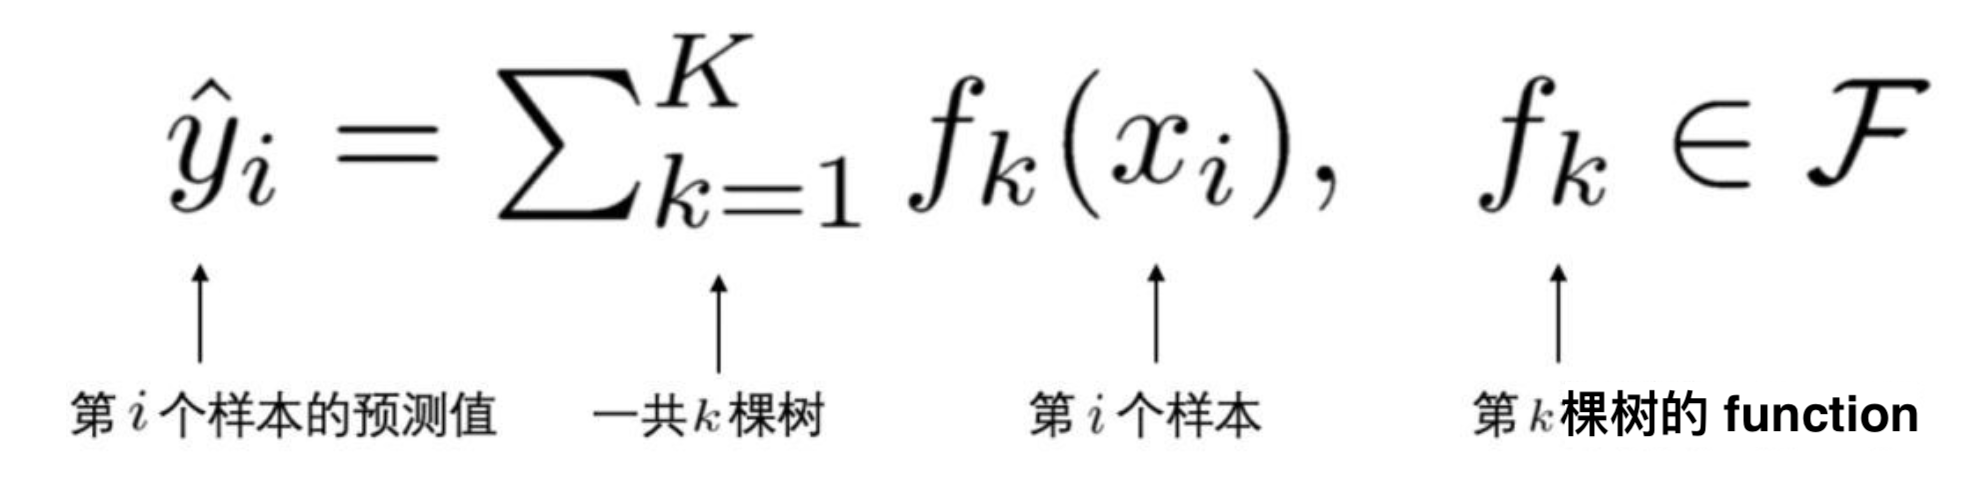
\includegraphics[width=.8\textwidth]{fig/XGBoost_Eq_Ith_Tree_Prediction.png}
\end{figure}
    \item 将全部$k$棵树的复杂度进行求和,添加到目标函数中作为正则化项,用于防止模型过度拟合;
\end{itemize}

\subsubsection{学习第$t$棵树}
XGBoost 是一个加法模型,假设我们第$t$次迭代要训练的树模型是 $f_t()$,则有:
\begin{figure}[H]
    \centering
    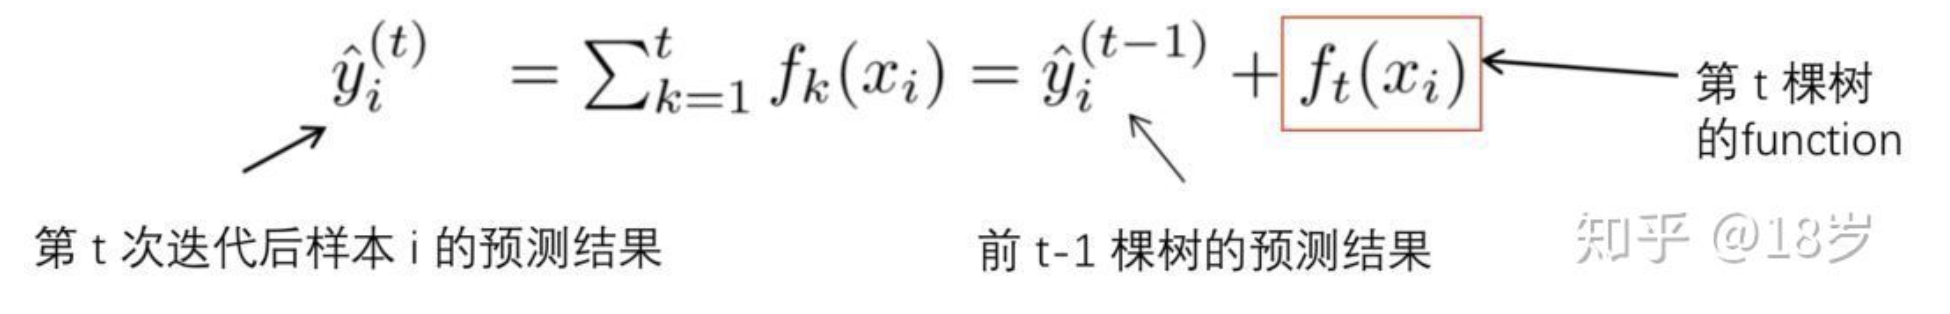
\includegraphics[width=.8\textwidth]{fig/XGBoost_Eq_Train_Tth_Tree.png}
\end{figure}

将上式带入目标函数 $Obj$ ,可以得到:
\begin{figure}[H]
    \centering
    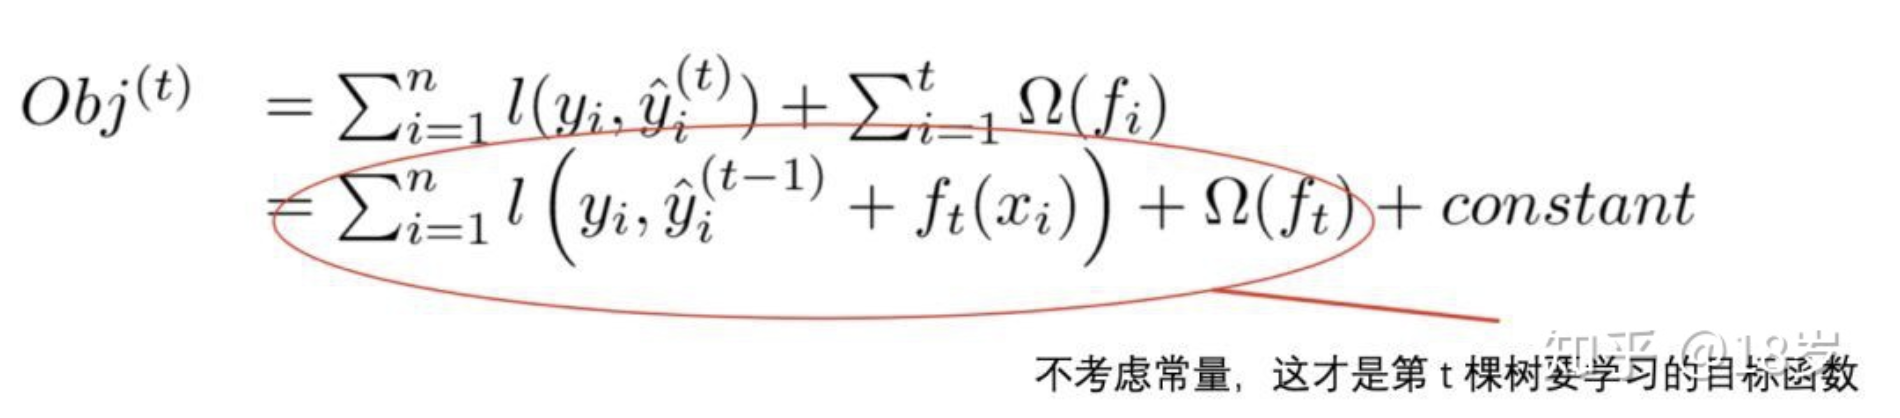
\includegraphics[width=.8\textwidth]{fig/XGBoost_Eq_Train_Tth_Tree_Objective.png}
\end{figure}

\begin{framed}
理解后面两项:

$\sum_{i=1}^t\Omega(f_i) = \sum_{i=1}^{t-1}\Omega(f_i) + \Omega(f_t) = constant + \Omega(f_t)$

也就是说,这里我们将正则化项进行了拆分,由于前 $t-1$ 棵树的结构已经确定,因此,前 $t-1$ 棵树的复杂度之和可以用一个常量 $constant$ 表示;只需要考虑第 $t$ 棵树的正则化项即可。
\end{framed}

注意上式中,只有一个变量,那就是第 $t$ 棵树 $f_t(x_i)$,其余的都是已知量或可通过已知量可以计算出来的。

\subsubsection{泰勒公式展开}
首先简单回忆一下,泰勒公式是将一个在 $x = x_0$ 处具有$n$阶导数的函数 $f(x)$ 利用关于 $(x-x_0)$ 的 $n$ 次多项式来逼近函数的方法。

泰勒公式的二阶展开形式如下:
$$
f(x + \Delta x) \backsimeq f(x) + f'(x)\Delta x + \frac{1}{2} f''(x) \Delta x^2
$$

\textbf{回到我们的问题上来,$f(x)$ 对应于我们的损失函数 $l$ ,$x$ 对应于前 $t-1$ 棵树的预测值,$\Delta x$ 对应于我们正在训练的第 $t$ 棵树}。


首先定义损失函数 $l$ 关于 $\hat{y}^{(t-1)}$ 的一阶偏导数和二阶偏导数(\textbf{注意这里的导是对$\hat{y}^{(t-1)}$ 求导}):
\begin{figure}[H]
    \centering
    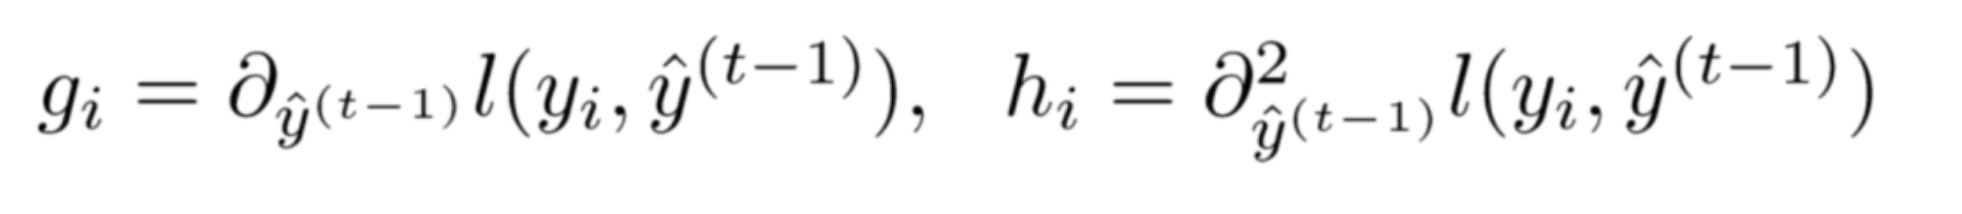
\includegraphics[width=.8\textwidth]{fig/XGBoost_Eq_Partial_Loss.png}
\end{figure}

那么,我们的\textbf{损失函数就可以转化为下式}(标出了与泰勒公式中$x$和$\Delta x$的对应关系):
\begin{figure}[H]
    \centering
    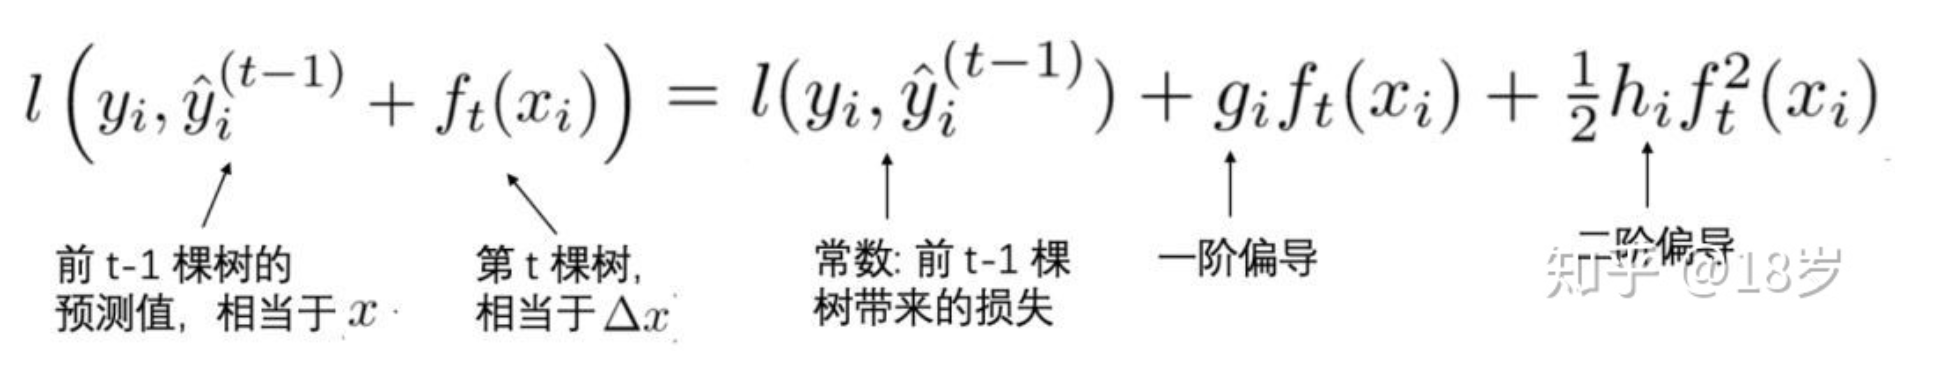
\includegraphics[width=.8\textwidth]{fig/XGBoost_Eq_Partial_Loss_Tylor.png}
\end{figure}

将上述二阶展开式,带入到目标函数 $Obj$ 中,可以得到目标函数 $Obj$ 的近似值:
\begin{figure}[H]
    \centering
    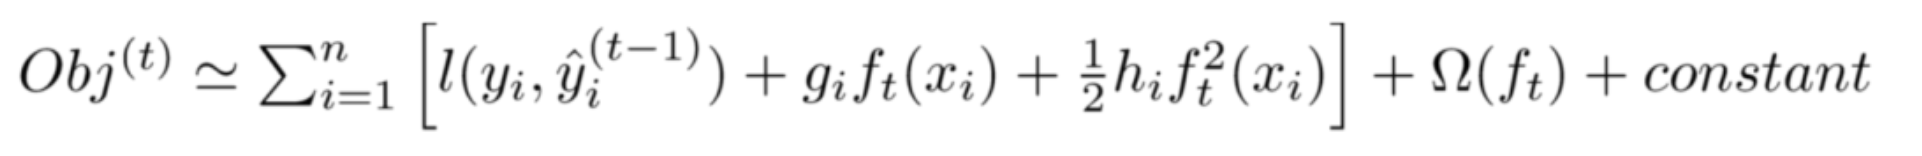
\includegraphics[width=.8\textwidth]{fig/XGBoost_Eq_Partial_Loss_Tylor_Obj.png}
\end{figure}

去掉全部常数项,得到目标函数:
\begin{figure}[H]
    \centering
    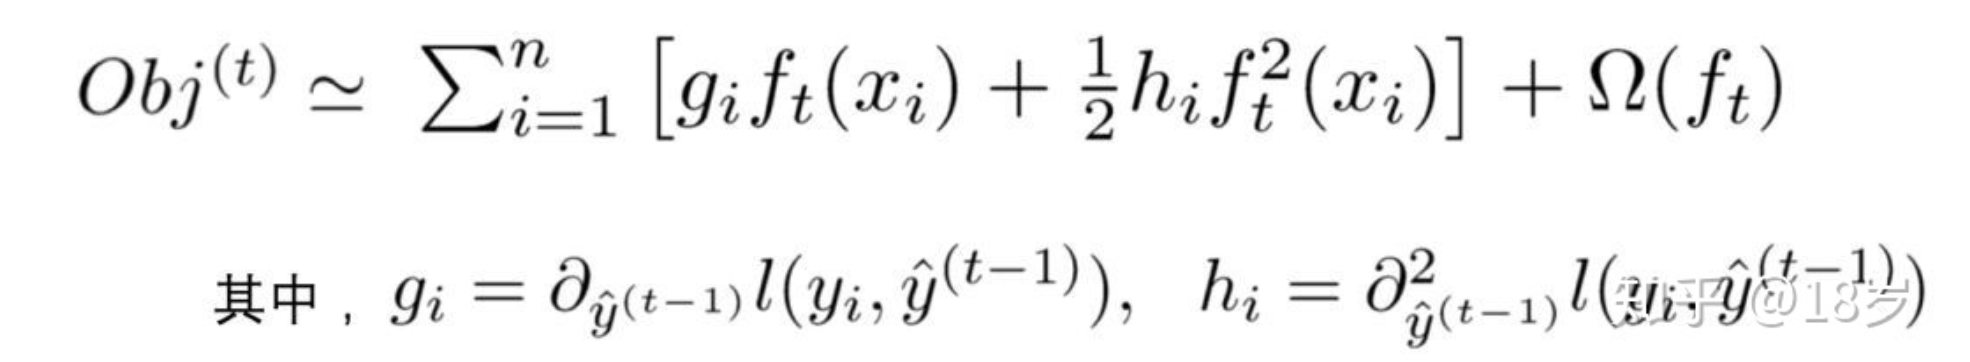
\includegraphics[width=.8\textwidth]{fig/XGBoost_Eq_Partial_Loss_Tylor_Obj_No_Constants.png}
\end{figure}

\begin{framed}
我们以平方损失函数为例:
$$
\sum_{i=1}^n\Bigg(y_i - \Big(\hat{y}^{(t-1)} + f_t(x_i)\Big)\Bigg)^2
$$

则:
$$
g_i = \frac{\partial \Big(\hat{y}^{(t-1)} - y_i\Big)^2}{\partial \hat{y}^{(t-1)}} = 2\Big(\hat{y}^{(t-1)} - y_i\Big)
$$

$$
h_i = \frac{\partial^2 \Big(\hat{y}^{(t-1)} - y_i\Big)^2}{\partial^2 \hat{y}^{(t-1)}} = 2
$$

由于在第 $t$ 步时$\hat{y}^{(t-1)}$其实是一个已知的值,所以$l(y, \hat{y}^{(t-1)})$是一个常数,其对函数的优化不会产生影响,因此目标函数可以写成:
$$
Obj^{(t)} \approx \sum_{i=1}^n\Bigg[ g_i f_t (x_i) + \frac{1}{2}h_if^2_t(x_i)\Bigg] + \sum_{i=1}^t\Omega(f_i)
$$


\end{framed}



\subsubsection{定义一颗树}
我们重新定义一颗树,包括两个部分:
\begin{itemize}
\setlength{\itemsep}{0pt}
\setlength{\parsep}{0pt}
\setlength{\parskip}{0pt}
    \item 叶子结点的权重向量 $\omega$ ;
    \item 实例 -> 叶子结点的映射关系 $q$(本质是树的分支结构);
\end{itemize}

一棵树的表达形式定义如下:
\begin{figure}[H]
    \centering
    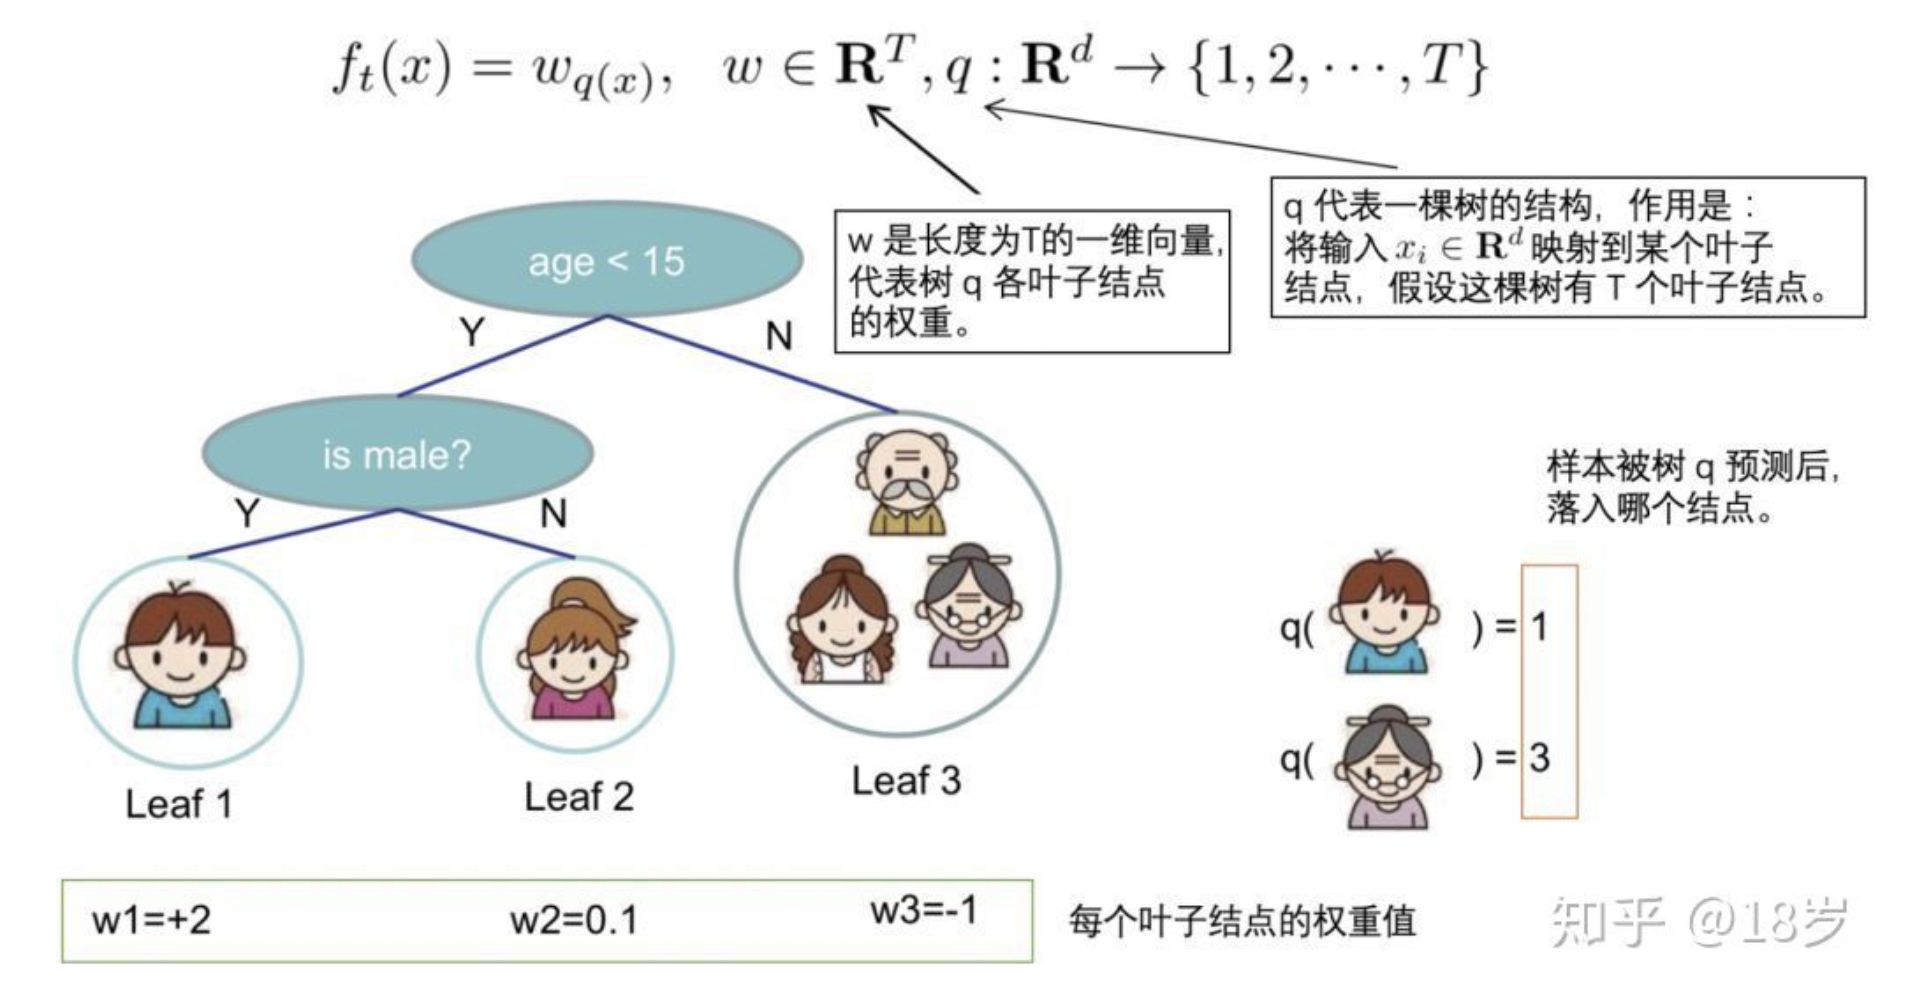
\includegraphics[width=1\textwidth]{fig/XGBoost_Tree_Definition_Example.png}
\end{figure}

\begin{framed}
加深理解:

\begin{itemize}
\setlength{\itemsep}{0pt}
\setlength{\parsep}{0pt}
\setlength{\parskip}{0pt}
    \item 输入的特征为 $d$ 维的向量 $x \in R^d$
    \item 将该特征向量映射到一个子树上,该子树共有$T$个子结点,每个结点有一个权重$w$,所以可以用一个$T$维的权重向量$w \in R^T$表示;
    \item 特征向量具体映射到哪个节点,由映射函数$q$表示,所以$q$的表达形式为:$q: R^d \Rightarrow \{1, 2, \cdots, T\}$
\end{itemize}
\end{framed}

\subsubsection{定义树的复杂度}
我们定义一颗树的复杂度 $\Omega$,它由两部分组成:
\begin{itemize}
\setlength{\itemsep}{0pt}
\setlength{\parsep}{0pt}
\setlength{\parskip}{0pt}
    \item 叶子结点的数量;
    \item 叶子结点权重向量的$L_2$范数;
\end{itemize}

\begin{figure}[H]
    \centering
    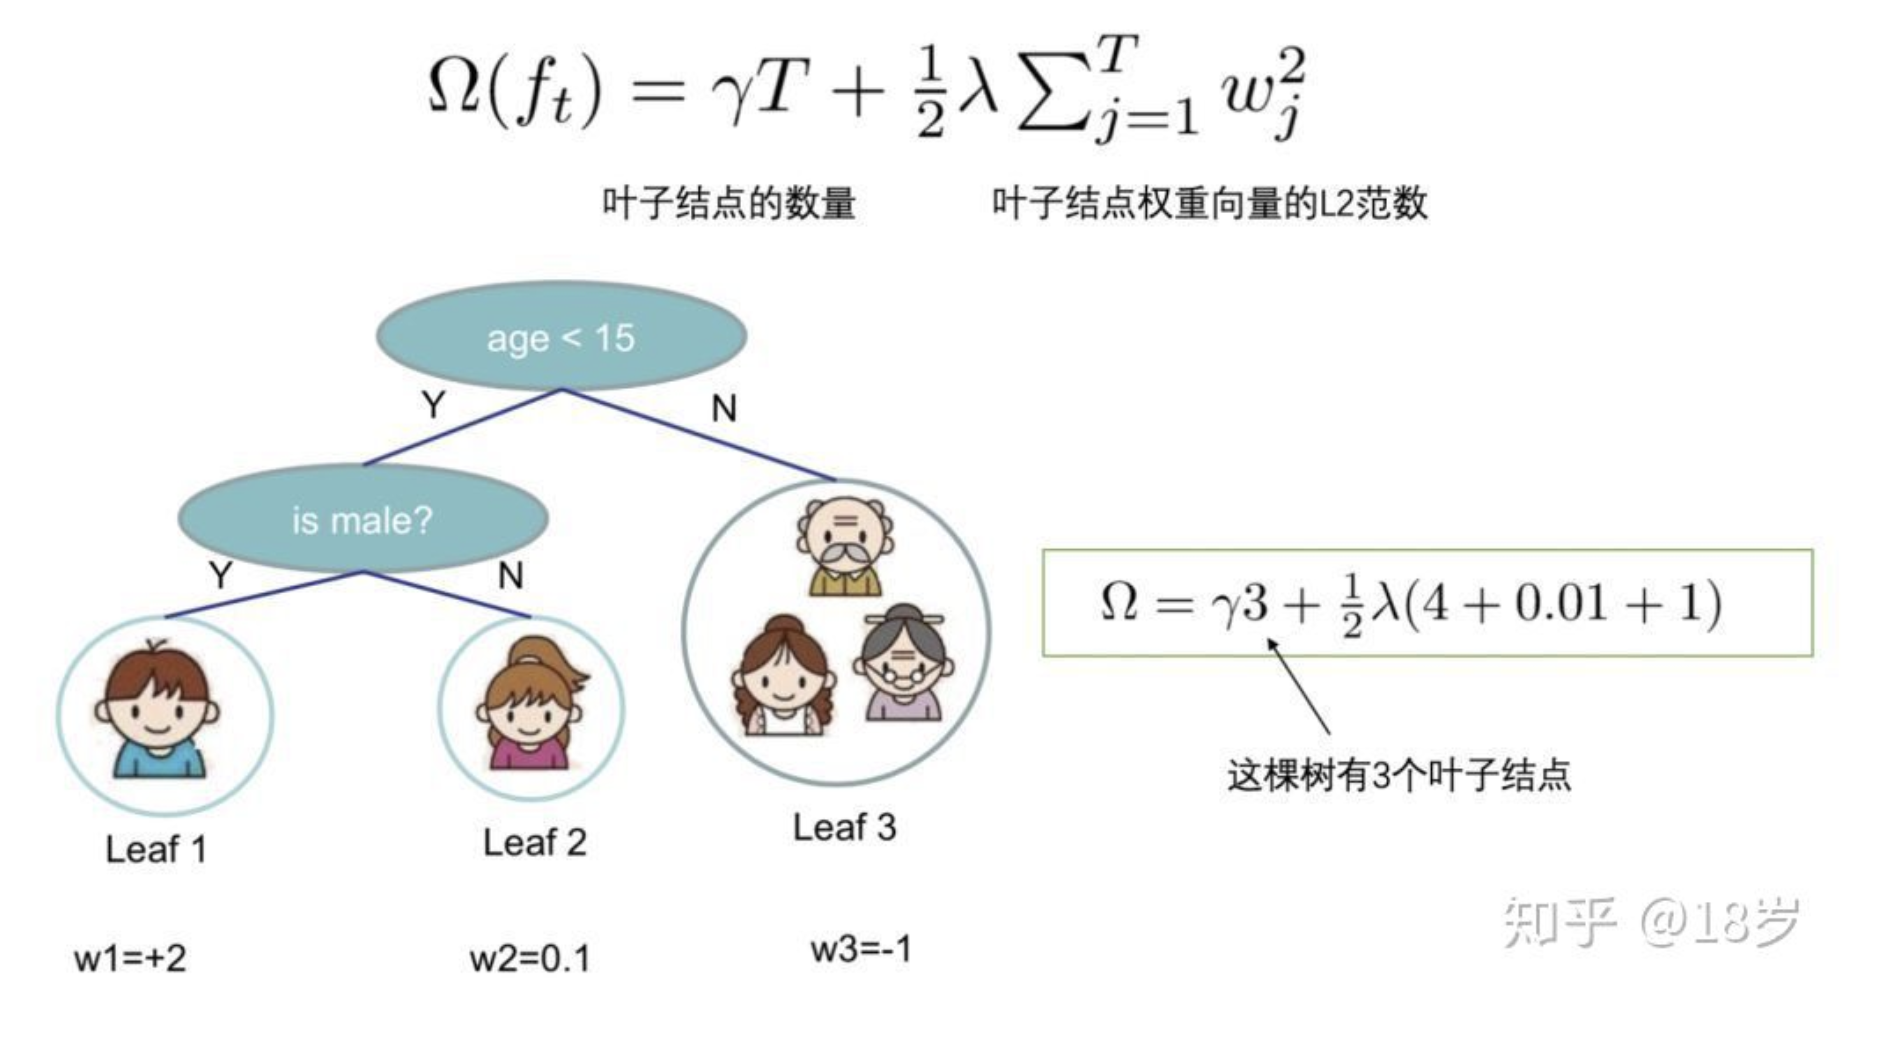
\includegraphics[width=1\textwidth]{fig/XGBoost_Tree_Complexity_Example.png}
\end{figure}

\subsubsection{叶子结点归组}
我们将属于第 $j$ 个叶子结点的所有样本 $x_i$ , 划入到一个叶子结点样本集中,数学表示如下:
\begin{figure}[H]
    \centering
    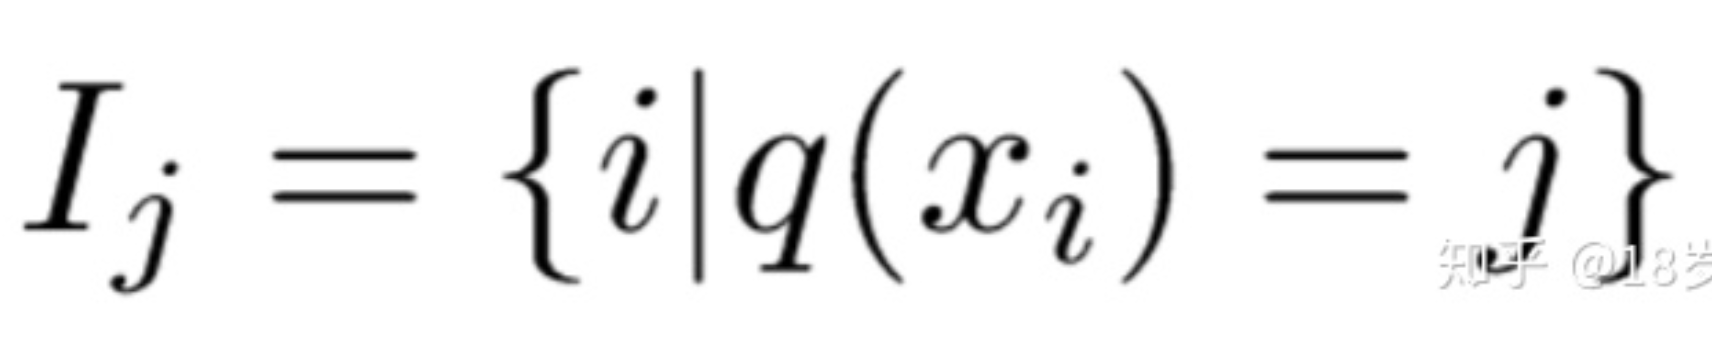
\includegraphics[width=.3\textwidth]{fig/XGBoost_Tree_Eq_Node_Grouping.png}
\end{figure}

然后,将树及其复杂度的定义,带入到泰勒展开后的目标函数$Obj$中,具体推导如下:
\begin{figure}[H]
    \centering
    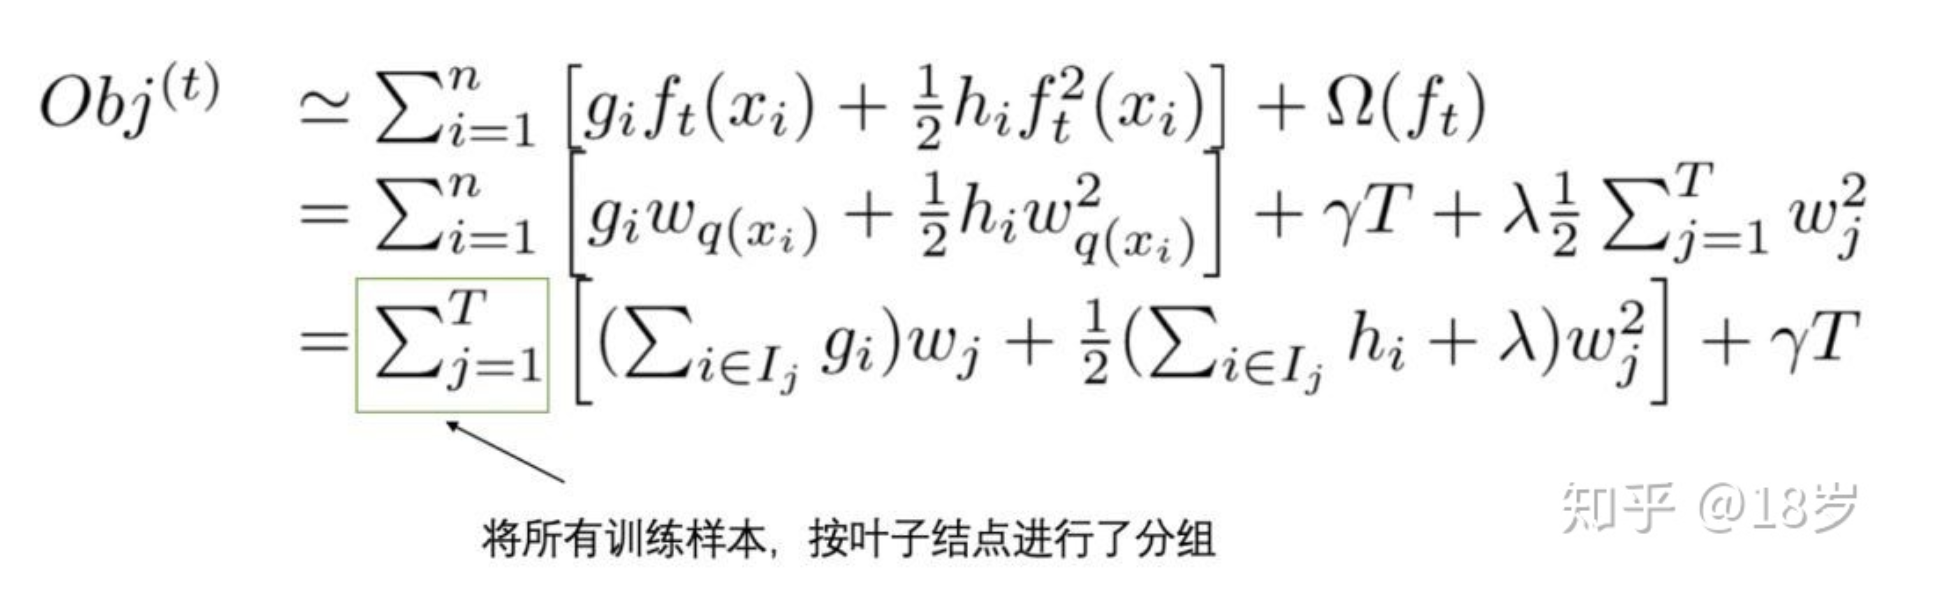
\includegraphics[width=.8\textwidth]{fig/XGBoost_Tree_Eq_Node_Grouping_Obj.png}
\end{figure}

为进一步简化该式,我们进行如下定义:
\begin{figure}[H]
    \centering
    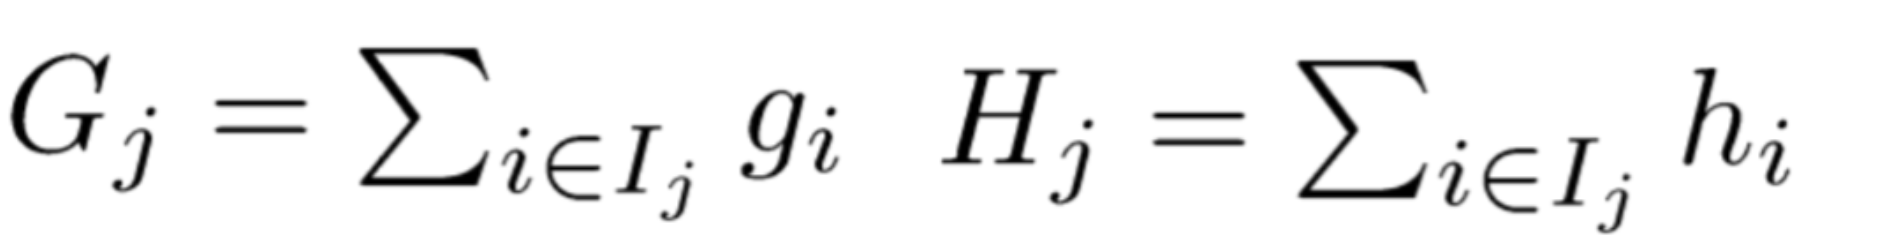
\includegraphics[width=.5\textwidth]{fig/XGBoost_Tree_Eq_Node_Grouping_Obj_Simplify.png}
\end{figure}

含义如下:
\begin{itemize}
\setlength{\itemsep}{0pt}
\setlength{\parsep}{0pt}
\setlength{\parskip}{0pt}
    \item $G_j$ :叶子结点 $j$ 所包含样本的\textbf{一阶偏导数累加之和},是一个常量;
    \item $H_j$ :叶子结点 $j$ 所包含样本的\textbf{二阶偏导数累加之和},是一个常量;
\end{itemize}

将 $G_j$ 和 $H_j$ 带入目标式 $Obj$,得到我们最终的目标函数(注意,此时式中的变量只剩下第 $t$ 棵树的权重向量 $W$):
\begin{figure}[H]
    \centering
    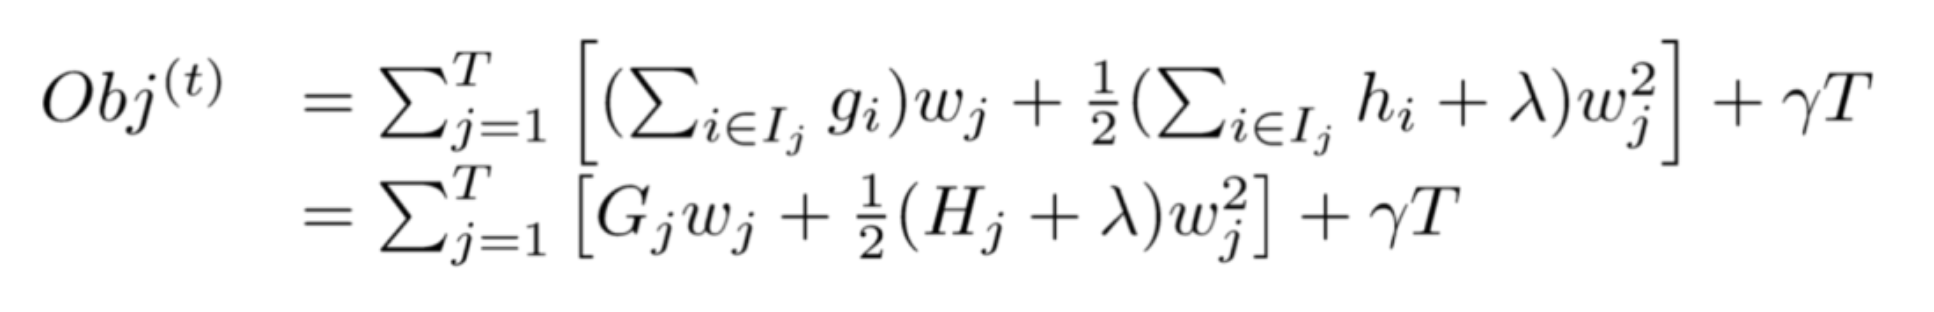
\includegraphics[width=.8\textwidth]{fig/XGBoost_Tree_Eq_Node_Grouping_Obj_Simplify_Final.png}
\end{figure}

\begin{framed}
给定训练特征后,$G_j, H_j$ 就确定下来了,所以是常量;只有 $W$ 是需要求解的。
\end{framed}

\subsubsection{树结构打分}
回忆一下高中数学知识。假设有一个一元二次函数,形式如下:
$$
Gx + \frac{1}{2}Hx^2, \qquad H > 0
$$

我们可以套用一元二次函数的最值公式轻易地求出最值点:
$$
x* = -\frac{G}{H}
$$
$$
y*  = -\frac{1}{2}\frac{G^2}{H}
$$

那回到我们的目标函数 $Obj$,该如何求出它的最值呢?
\begin{figure}[H]
    \centering
    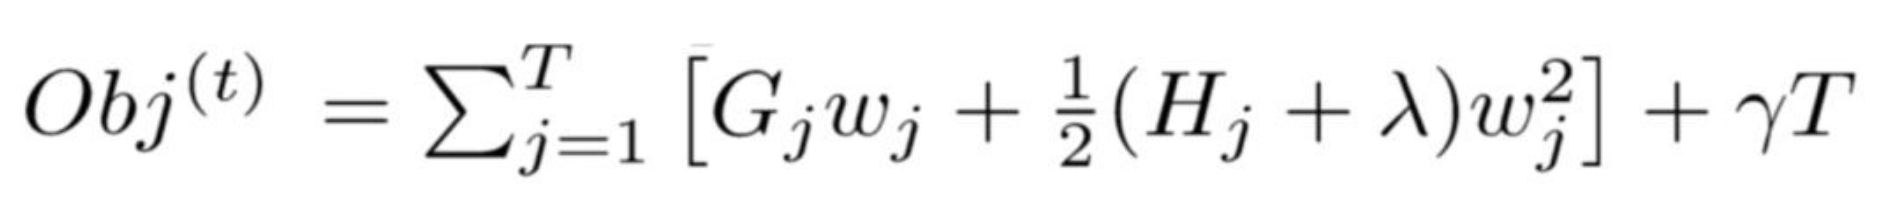
\includegraphics[width=.8\textwidth]{fig/XGBoost_Tree_Eq_Node_Grouping_Obj_Final.png}
\end{figure}

先简单分析一下上面的式子。对于每个叶子结点 $j$ , 可以将其从目标式 $Obj$ 中拆解出来:
\begin{figure}[H]
    \centering
    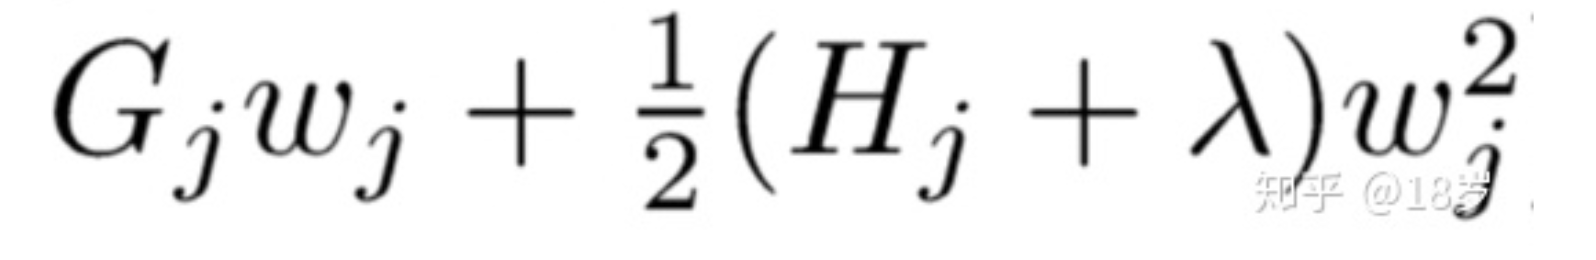
\includegraphics[width=.4\textwidth]{fig/XGBoost_Tree_Eq_Node_Grouping_Obj_Final_Decompose.png}
\end{figure}

在上面我们提到,$G_j$ 和 $H_j$ 相对于第 $t$ 棵树来说是可以计算出来的。那么,这个式子就是一个只包含一个变量叶子结点权重$w_j$ 的一元二次函数,上面也提到了,我们可以通过最值公式求出它的最值点。

再次分析一下目标函数$Obj$,可以发现,各个叶子结点的目标子式是相互独立的,也就是说,当每个叶子结点的子式都达到最值点时,整个目标函数式$Obj$才达到最值点。

那么,\textbf{假设目前树的结构已经固定},套用一元二次函数的最值公式,我们可以轻易求出,每个叶子结点的权重 $w^*_j$ 及其此时达到最优的 $Obj$ 的目标值:
\begin{figure}[H]
    \centering
    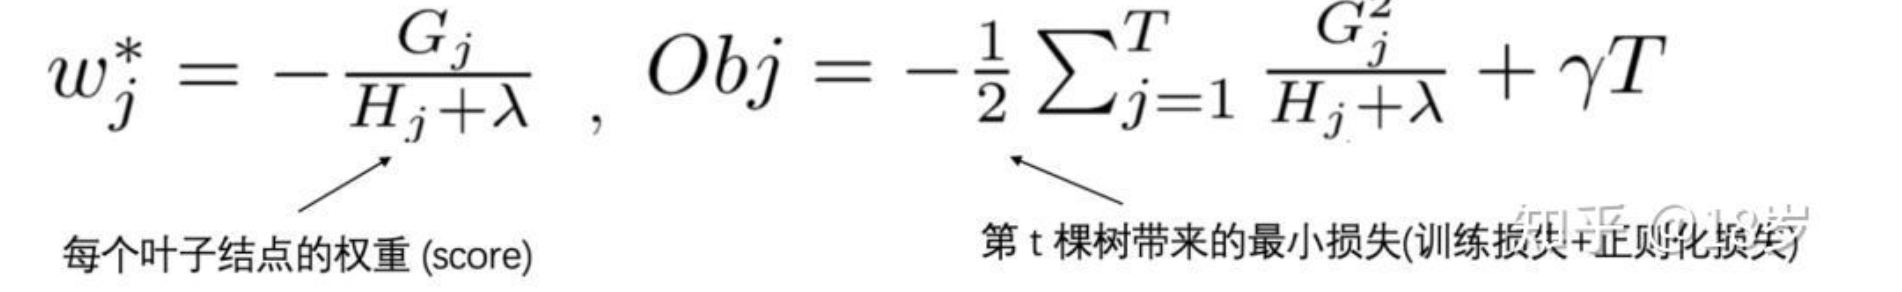
\includegraphics[width=.8\textwidth]{fig/XGBoost_Tree_Eq_Node_Grouping_Obj_Final_Opt.png}
\end{figure}

\begin{framed}
\textbf{实例演示}
\begin{figure}[H]
    \centering
    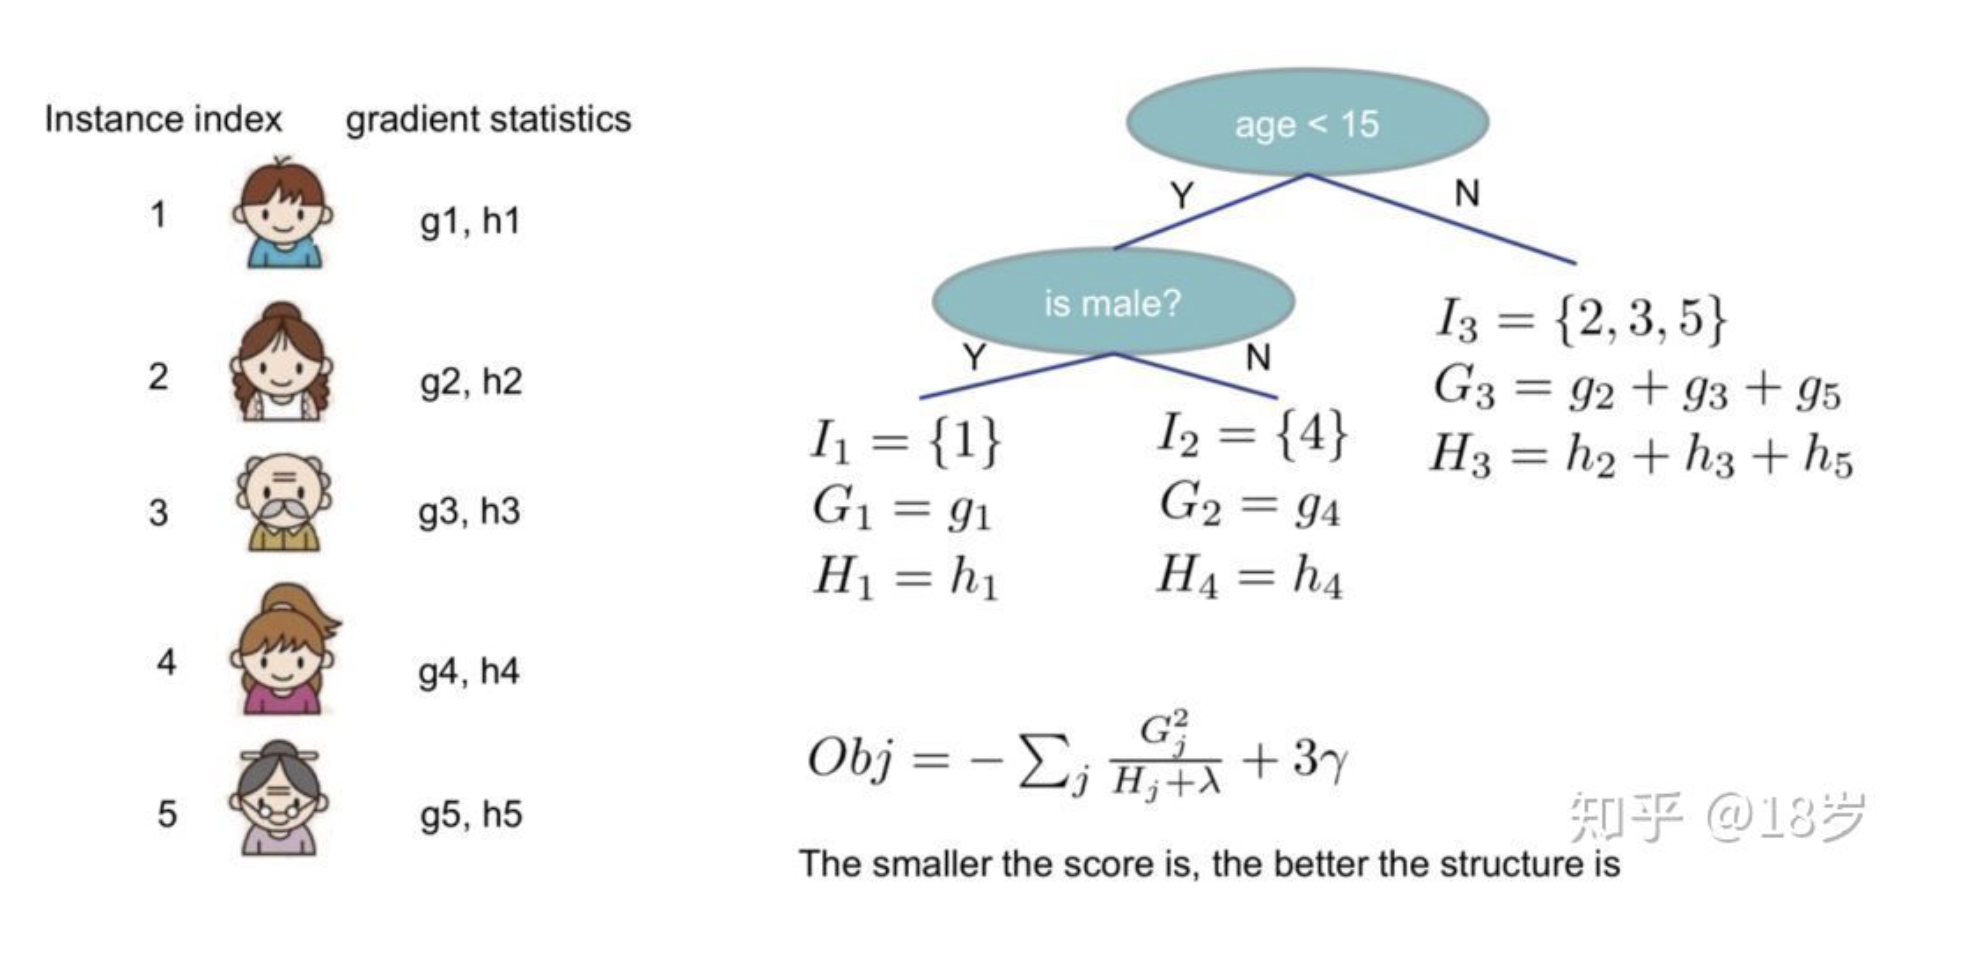
\includegraphics[width=1\textwidth]{fig/XGBoost_Tree_Train_Example.png}
\end{figure}
\end{framed}

\begin{framed}
\textbf{与 GBDT 的比较}
\url{https://zhuanlan.zhihu.com/p/82671707}

XGBoost 更新 $w_j$ 的公式为:
$$
w_j = \frac{\sum_{i\in I_j}g(x_i)}{\sum_{i\in I_j}h(x_i) + \lambda}
$$

这里我们和传统的gbdt做对比,传统的gbdt的叶节点值是这样的:
$$
w_j = \frac{\sum_{i\in I_j}g(x_i)}{\sum_{i\in I_j}1}
$$

传统的gbdt的基树是cart tree,\textbf{叶节点值的预测输出是这个叶节点值的所有样本的标签的平均值},单纯从单个cart tree的角度(不涉及gbm框架)来说,如果是回归问题,某个叶子节点的预测输出就是这个叶子节点所有样本的标签值的平均,比如说回归问题中某个叶子节点所有的样本的标签是[0.5,0.4,0.0],则预测输出就是三者的平均0.3,传统的gbdt也是一样的,只不过每一轮要拟合的标签值是前面所有所有tree预测结果与真实标签值计算出来的负梯度而已,比如第$t$轮,某个叶子节点的值为[0.3,0.4,0.2](这里的值是上一轮拟合得到的损失函数的负梯度),则预测输出就是简单的求平均0.3。也就是上面的这个式子。

而xgboost通过复杂的推导最后得出结论,叶子节点值不应该是简单的上一轮负梯度的均值,应该加入二阶负梯度和树的正则化系数,于是就得到了上面的公式。

\textbf{区别就是:分母不再是简单平均而是变成了损失函数二阶梯度的求和+树的正则化系数}。
\end{framed}

\subsection{一棵树的生长细节}
\subsubsection{分裂一个结点}
在实际训练过程中,当建立第 $t$ 棵树时,XGBoost支持采用\textbf{贪心法和近似算法}进行树结点的分裂;

\textbf{(1). 贪心算法}

从树深为0时开始:
\begin{itemize}
\setlength{\itemsep}{0pt}
\setlength{\parsep}{0pt}
\setlength{\parskip}{0pt}
    \item 对树中的每个叶子结点尝试进行分裂;
    \item 每次分裂后,原来的一个叶子结点继续分裂为左右两个子叶子结点,原叶子结点中的样本集将根据该结点的判断规则分散到左右两个叶子结点中;
    \item 新分裂一个结点后,我们需要检测这次分裂是否会给损失函数带来增益,增益的定义如下:
    \begin{figure}[H]
    \centering
    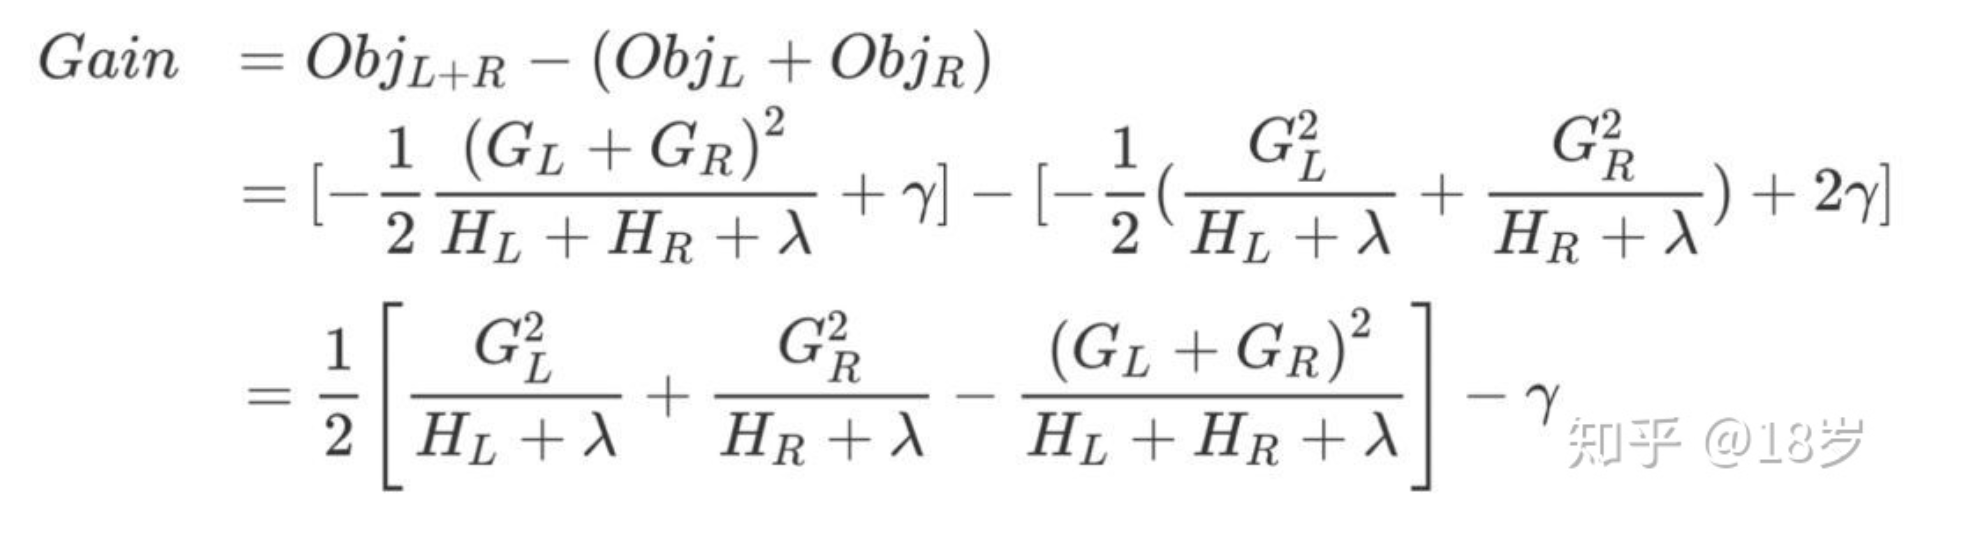
\includegraphics[width=1\textwidth]{fig/XGBoost_Tree_Eq_Node_Split_Gain.png}
	\end{figure}
\end{itemize}

如果增益 Gain>0,即分裂为两个叶子节点后,目标函数下降了,那么我们会考虑此次分裂的结果。

但是,在一个结点分裂时,可能有很多个分裂点,每个分裂点都会产生一个增益,如何才能寻找到最优的分裂点呢?接下来会讲到。

\textbf{(2). 近似算法}
贪婪算法可以的到最优解,但当数据量太大时则无法读入内存进行计算,近似算法主要针对贪婪算法这一缺点给出了近似最优解。

对于每个特征,只考察分位点可以减少计算复杂度。

该算法会首先根据特征分布的分位数提出候选划分点,然后将连续型特征映射到由这些候选点划分的桶中,然后聚合统计信息找到所有区间的最佳分裂点。

在提出候选切分点时有两种策略:Global:学习每棵树前就提出候选切分点,并在每次分裂时都采用这种分割;Local:每次分裂前将重新提出候选切分点。

直观上来看,Local 策略需要更多的计算步骤,而 Global 策略因为节点没有划分所以需要更多的候选点。

\subsubsection{寻找最佳分裂点}
在分裂一个结点时,我们会有很多个候选分割点,寻找最佳分割点的大致步骤如下:
\begin{itemize}
\setlength{\itemsep}{0pt}
\setlength{\parsep}{0pt}
\setlength{\parskip}{0pt}
    \item 遍历每个结点的每个特征;
    \item 对每个特征,按特征值大小将特征值排序;
    \item 线性扫描,找出每个特征的最佳分裂特征值;
    \item 在所有特征中找出最好的分裂点(分裂后增益最大的特征及特征值)。
\end{itemize}

上面是一种贪心的方法,每次进行分裂尝试都要遍历一遍全部候选分割点,也叫做全局扫描法。但当数据量过大导致内存无法一次载入或者在分布式情况下,贪心算法的效率就会变得很低,全局扫描法不再适用。基于此,XGBoost提出了一系列加快寻找最佳分裂点的方案:

\begin{itemize}
\setlength{\itemsep}{0pt}
\setlength{\parsep}{0pt}
\setlength{\parskip}{0pt}
    \item \textbf{特征预排序+缓存}:XGBoost在训练之前,预先对每个特征按照特征值大小进行排序,然后保存为block结构,后面的迭代中会重复地使用这个结构,使计算量大大减小;
    \item \textbf{分位点近似法}:对每个特征按照特征值排序后,采用类似分位点选取的方式,仅仅选出常数个特征值作为该特征的候选分割点,在寻找该特征的最佳分割点时,从候选分割点中选出最优的一个;
    \item \textbf{并行查找}:由于各个特性已预先存储为block结构,XGBoost支持\textbf{利用多个线程并行地计算每个特征的最佳分割点},这不仅大大提升了结点的分裂速度,也极利于大规模训练集的适应性扩展。
\end{itemize}

\subsubsection{停止生长}
一棵树不会一直生长下去,下面是一些常见的限制条件。

(1) 当新引入的一次分裂所带来的增益Gain<0时,放弃当前的分裂。这是训练损失和模型结构复杂度的博弈过程。
\begin{figure}[H]
    \centering
    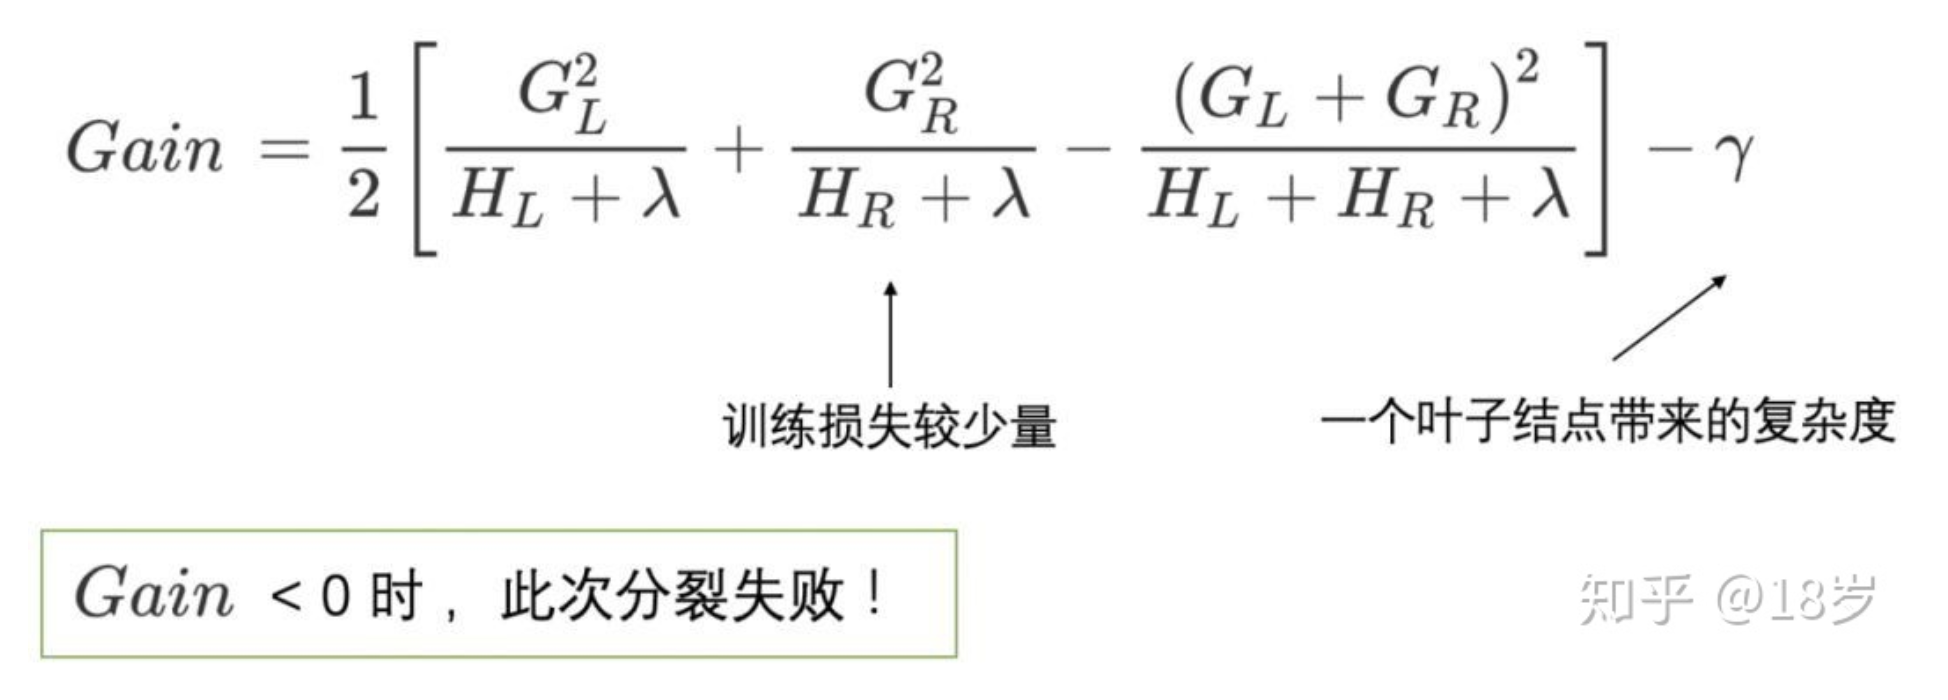
\includegraphics[width=1\textwidth]{fig/XGBoost_Tree_Eq_Node_Split_Stop_1.png}
\end{figure}

(2) 当树达到最大深度时,停止建树,因为树的深度太深容易出现过拟合,这里需要设置一个\textbf{超参数 max\_depth}。

(3) 当引入一次分裂后,重新计算新生成的左、右两个叶子结点的样本权重和。如果任一个叶子结点的样本权重低于某一个阈值,也会放弃此次分裂。这涉及到一个\textbf{超参数: 最小样本权重和},是指如果一个叶子节点包含的样本数量太少也会放弃分裂,防止树分的太细,这也是过拟合的一种措施。

每个叶子结点的样本权值和计算方式如下:
$$
w^*_j = -\frac{G_j}{H_j + \lambda}
$$

\subsection{工程实现}
\subsubsection{块结构设计}
我们知道,\textbf{决策树的学习最耗时的一个步骤就是在每次寻找最佳分裂点是都需要对特征的值进行排序}。而 XGBoost 在训练之前对根据特征对数据进行了排序,然后保存到块结构中,并在每个块结构中都采用了稀疏矩阵存储格式(Compressed Sparse Columns Format,CSC)进行存储,后面的训练过程中会重复地使用块结构,可以大大减小计算量。
\begin{itemize}
\setlength{\itemsep}{0pt}
\setlength{\parsep}{0pt}
\setlength{\parskip}{0pt}
    \item 每一个块结构包括一个或多个已经排序好的特征;
    \item 缺失特征值将不进行排序;
    \item 每个特征会存储指向样本梯度统计值的索引,方便计算一阶导和二阶导数值;
\end{itemize}

这种块结构存储的特征之间相互独立,方便计算机进行并行计算。在对节点进行分裂时需要选择增益最大的特征作为分裂,这时各个特征的增益计算可以同时进行,这也是 Xgboost 能够实现分布式或者多线程计算的原因。

\subsubsection{缓存访问优化算法}
块结构的设计可以减少节点分裂时的计算量,但特征值通过索引访问样本梯度统计值的设计会导致访问操作的内存空间不连续,这样会造成缓存命中率低,从而影响到算法的效率。

为了解决缓存命中率低的问题,XGBoost 提出了缓存访问优化算法:为每个线程分配一个连续的缓存区,将需要的梯度信息存放在缓冲区中,这样就是实现了非连续空间到连续空间的转换,提高了算法效率。

此外适当调整块大小,也可以有助于缓存优化。

\subsubsection{“核外”块计算}
当数据量过大时无法将数据全部加载到内存中,只能先将无法加载到内存中的数据暂存到硬盘中,直到需要时再进行加载计算,而这种操作必然涉及到因内存与硬盘速度不同而造成的资源浪费和性能瓶颈。为了解决这个问题,XGBoost 独立一个线程专门用于从硬盘读入数据,以实现处理数据和读入数据同时进行。

此外,XGBoost 还用了两种方法来降低硬盘读写的开销:块压缩:对 Block 进行按列压缩,并在读取时进行解压;块拆分:将每个块存储到不同的磁盘中,从多个磁盘读取可以增加吞吐量。

\subsection{总结:XGBoost 推导}
\begin{figure}[H]
    \centering
    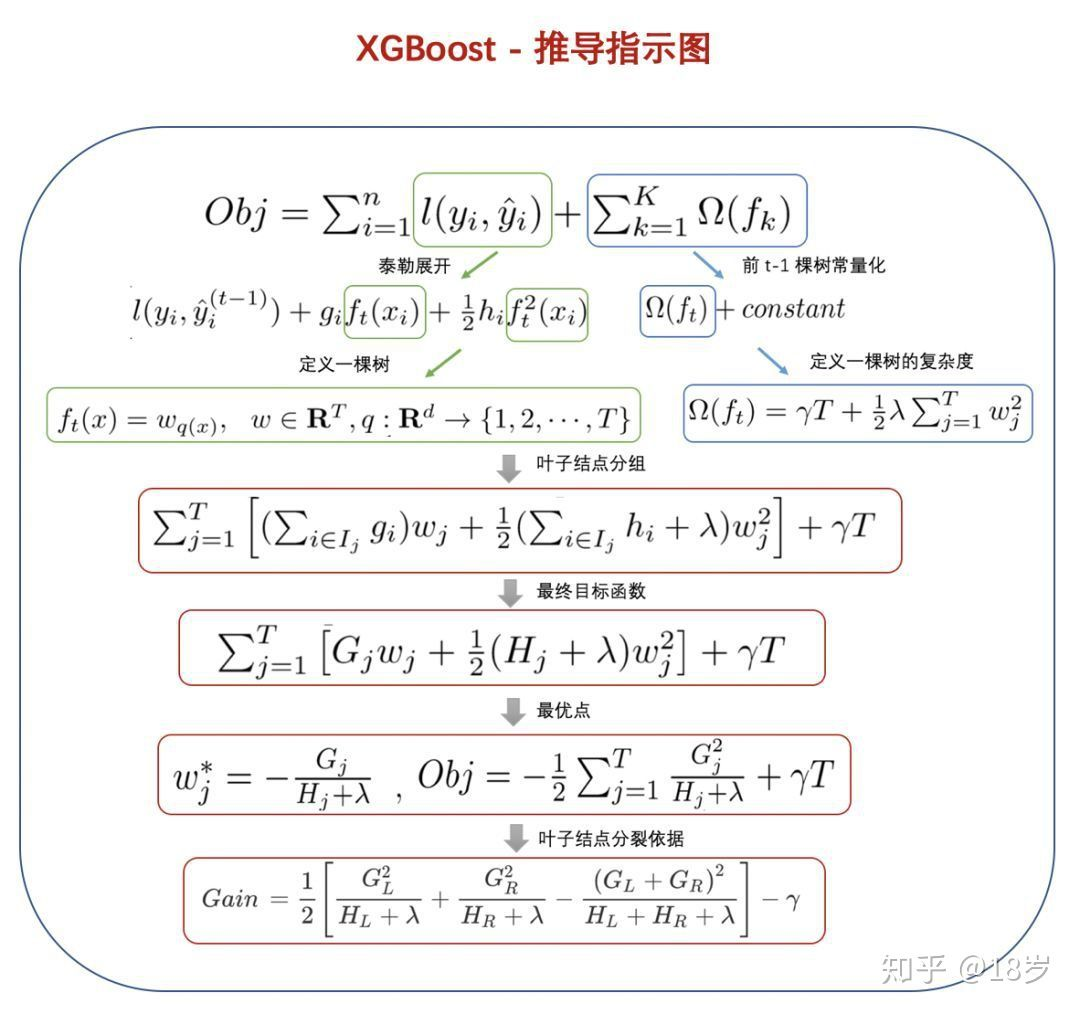
\includegraphics[width=1\textwidth]{fig/XGBoost_Eq_Conclusion.jpg}
\end{figure}

\section{XGBoost 的 python 实现\cite{XGBoost_In_Python}}
\subsection{构建XGBoost}
参数说明:
\begin{itemize}
\setlength{\itemsep}{0pt}
\setlength{\parsep}{0pt}
\setlength{\parskip}{0pt}
    \item n\_estimators: int,树的数量
    \item learning\_rate: float,梯度下降的学习率
    \item min\_samples\_split: int,每棵子树的节点的最小数目(小于后不继续切割)
    \item min\_impurity: float, 每颗子树的最小纯度(小于后不继续切割)
    \item max\_depth: int,每颗子树的最大层数(大于后不继续切割)
\end{itemize}

损失函数定义如下:
\begin{python}
class LeastSquaresLoss():
    """Least squares loss"""

    def gradient(self, actual, predicted):
        return actual - predicted

    def hess(self, actual, predicted):
        return np.ones_like(actual)
\end{python}

XGBoost 的 Tree 的定义如下:
\begin{python}
from decision_tree.decision_tree_model import DecisionTree

class XGBoostRegressionTree(DecisionTree):
    def _split(self, y):
        """ y contains y_true in left half of the middle column and
        y_pred in the right half. Split and return the two matrices """

        col = int(np.shape(y)[1]/2)
        y, y_pred = y[:, :col], y[:, col:]
        return y, y_pred
 
    def _gain(self, y, y_pred):
        nominator = np.power((self.loss.gradient(y, y_pred)).sum(), 2)
        denominator = self.loss.hess(y, y_pred).sum()
        return 0.5 * (nominator / denominator)
 
    def _gain_by_taylor(self, y, y1, y2):
        # Split
        y, y_pred = self._split(y)
        y1, y1_pred = self._split(y1)
        y2, y2_pred = self._split(y2)
 
        true_gain = self._gain(y1, y1_pred)
        false_gain = self._gain(y2, y2_pred)
        gain = self._gain(y, y_pred)
        return true_gain + false_gain - gain
 
    def _approximate_update(self, y):
        # y split into y, y_pred
        y, y_pred = self._split(y)
        gradient = np.sum(self.loss.gradient(y, y_pred),axis=0)
        hessian = np.sum(self.loss.hess(y, y_pred), axis=0)
        update_approximation =  gradient / hessian
        return update_approximation
 
 
    def fit(self, X, y):
        self._impurity_calculation = self._gain_by_taylor
        self._leaf_value_calculation = self._approximate_update
        super(XGBoostRegressionTree, self).fit(X, y)
\end{python}

XGBoost 的 python 实现如下:

\begin{python}
class XGBoost(object):
	def __init__(self, n_estimators=200, learning_rate=0.01, min_samples_split=2,min_impurity=1e-7, max_depth=2):
        self.n_estimators = n_estimators  # Number of trees
        #…… 初始化参数部分 ……
        
        self.bar = progressbar.ProgressBar(widgets=bar_widgets)
	     
        # Log loss for classification 初始化损失函数
        self.loss = LeastSquaresLoss()
 
        # Initialize regression trees 初始化回归树集合(**注意,会先初始化生成所有树**)
        self.trees = []
        for _ in range(n_estimators):
            tree = XGBoostRegressionTree(
                min_samples_split=self.min_samples_split,
                min_impurity=min_impurity,
                max_depth=self.max_depth,
                loss=self.loss)
            self.trees.append(tree)

    def fit(self, X, y):
        # y = to_categorical(y)
        m = X.shape[0] #m 是 X(训练样本) 的个数
        y = np.reshape(y, (m, -1))  # (m,-1)表示 m 行,列数与原来相同
        y_pred = np.zeros(np.shape(y)) #预测值全部置为0
        # 遍历所有树
        for i in self.bar(range(self.n_estimators)):
            tree = self.trees[i]
            y_and_pred = np.concatenate((y, y_pred), axis=1)
            tree.fit(X, y_and_pred) 
            update_pred = tree.predict(X) #计算预测值
            update_pred = np.reshape(update_pred, (m, -1))
            y_pred += update_pred #更新预测值,**累加残差**
            
    def predict(self, X):
        y_pred = None
        m = X.shape[0]
        # Make predictions
        for tree in self.trees:
            # Estimate gradient and update prediction
            update_pred = tree.predict(X)
            update_pred = np.reshape(update_pred, (m, -1))
            if y_pred is None:
                y_pred = np.zeros_like(update_pred)
            y_pred += update_pred
        return y_pred
\end{python}

\subsection{代码思路总结}
1. 初始化生成指定数量(n\_estimators)的树集合;

2. 对每棵子树,传入训练集$X$和标注集$y$,训练该子树的参数;

2.1. 通过 gain() 函数计算切分后的数据集的gain 值(代码中忽略了 $\lambda$):
$$
\frac{G_i^2}{H_j^2+\lambda}
$$

其中:$G_i = \sum_{i \in I_j} g_i, H_j = \sum_{i \in I_j}h_i$

2.2 通过 gain\_by\_taylor() 来计算树节点的纯度,并以此来作为该子树是否要被分割的标准
\begin{figure}[H]
    \centering
    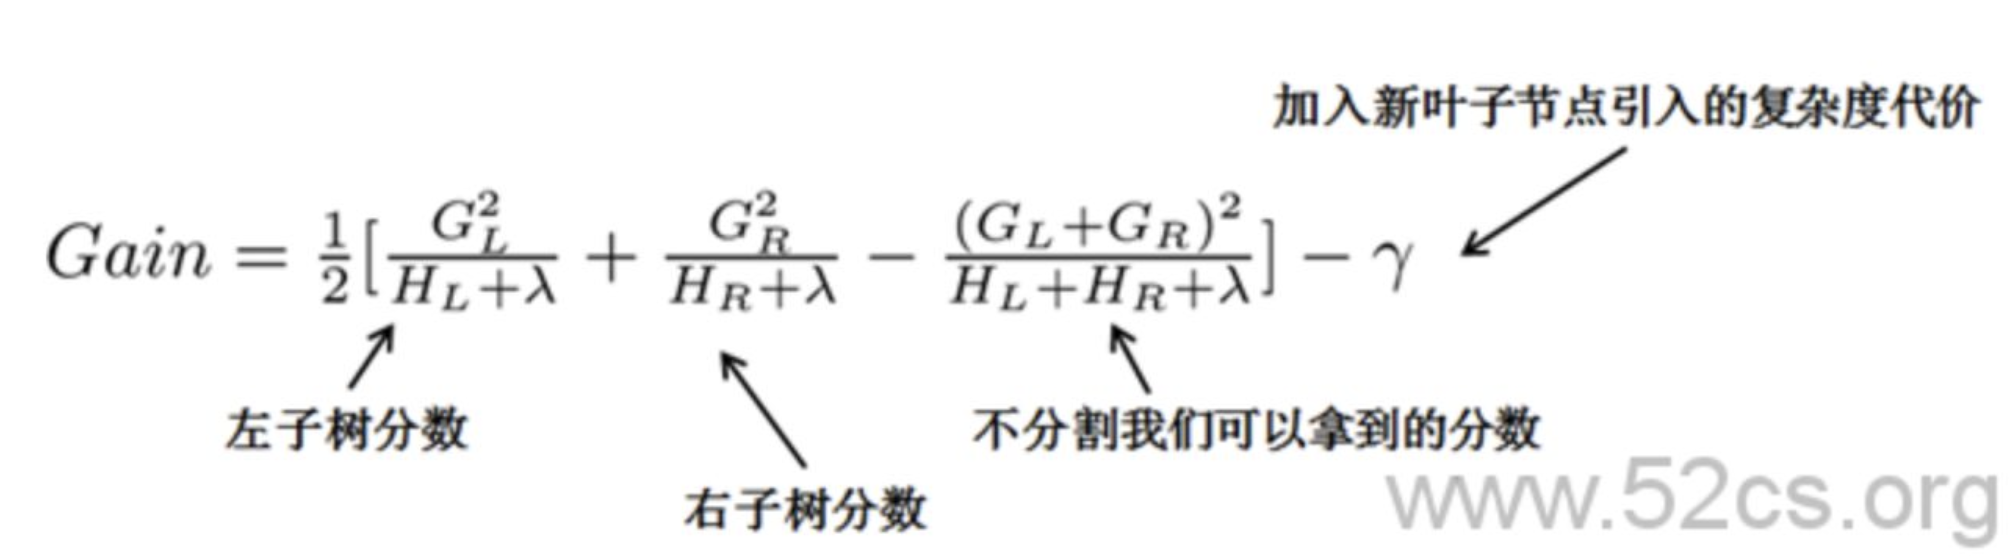
\includegraphics[width=1\textwidth]{fig/XGBoost_In_Python_Gain_by_taylor.png}
\end{figure}

2.3 该子树被切割完成后,每个子节点的取都是定好的了,通过 approximate\_update() 计算权重(代码中忽略了 $\lambda$ ):
$$
w_j = \frac{G_i^2}{H_j^2+\lambda}
$$

2.1.4 fit():将 gain\_by\_taylor() 作为切割树的标准;将approximate\_update()作为估算子节点取值的方法;传递回给DecisionTree,并以此来构建决策树;DecisionTree 的定义见:\url{https://github.com/RRdmlearning/Machine-Learning-From-Scratch/blob/master/decision_tree/decision_tree_model.py}

\section{LightGBM\cite{LightGBM_In_30_Minutes}}
\subsection{LightGBM和XGBoost对比}
LightGBM可以看成是XGBoost的升级加强版本,2017年经微软推出后,便成为各种数据竞赛中刷分夺冠的神兵利器。正如其名字中的Light所蕴含的那样,和XGBoost相比,LightGBM在大规模数据集上跑起来更加轻盈。

\begin{itemize}
\setlength{\itemsep}{0pt}
\setlength{\parsep}{0pt}
\setlength{\parskip}{0pt}
    \item \textbf{模型精度}:XGBoost和LightGBM相当。
    \item \textbf{训练速度}:LightGBM远快于XGBoost。
    \item \textbf{内存消耗}:LightGBM远小于XGBoost。
    \item \textbf{缺失值特征}:XGBoost和LightGBM都可以自动处理特征缺失值。
    \item \textbf{分类特征}:XGBoost不支持类别特征,需要OneHot编码预处理。LightGBM直接支持类别特征。
\end{itemize}

\subsection{LightGBM性能优化原理概述}
\subsubsection{XGBoost 的复杂度}
XGBoost模型训练的总体的复杂度可以粗略估计为:

\textbf{训练复杂度 = 树的棵数 $\times$ 每棵树上叶子的数量 $\times$ 生成每片叶子的复杂度}

由于XGBoost采用的基模型是二叉树,因此生成每片叶子需要分裂一次。而每次分裂,需要遍历所有特征上所有候选分裂点位,计算按照这些候选分裂点位分裂后的全部样本的目标函数增益,找到最大的那个增益对应的特征和候选分裂点位,从而生成一片新叶子。

生成一片叶子的复杂度可以粗略估计为:

\textbf{生成一片叶子的复杂度 = 特征数量 $\times$ 候选分裂点数量 $\times$ 样本的数量}

\subsubsection{LightGBM 的优化点}
LightGBM在XGBoost上主要有3方面的优化:Histogram、GOSS、EFB。

可以用如下一个简单公式来说明LightGBM和XGBoost的关系:

\textbf{LightGBM = XGBoost + Histogram + GOSS + EFB}

具体如下:
\begin{itemize}
\setlength{\itemsep}{0pt}
\setlength{\parsep}{0pt}
\setlength{\parskip}{0pt}
    \item Histogram算法:直方图算法,主要作用是减少候选分裂点数量;
    \item GOSS算法:基于梯度的单边采样算法,主要作用是减少样本的数量;
    \item EFB算法:互斥特征捆绑算法,作用是减少特征的数量。
\end{itemize}

通过这3个算法的引入,LightGBM生成一片叶子需要的复杂度大大降低了,从而极大节约了计算时间;同时Histogram算法还将特征由浮点数转换成0~255位的整数进行存储,从而极大节约了内存存储。

\subsection{Histogram算法}
直方图算法是替代XGBoost的预排序(pre-sorted)算法的。

预排序算法首先将样本按照特征取值排序,然后从全部特征取值中找到最优的分裂点位,该算法的候选分裂点数量与样本数量成正比。

而直方图算法通过将连续特征值离散化到固定数量(如255个)的bins上,使得候选分为点位为常数个(num\_bins -1).

此外,直方图算法还能够作直方图差加速。当节点分裂成两个时,右边叶子节点的直方图等于其父节点的直方图减去左边叶子节点的直方图。从而大大减少构建直方图的计算量。

预排序算法如下:
\begin{figure}[H]
    \centering
    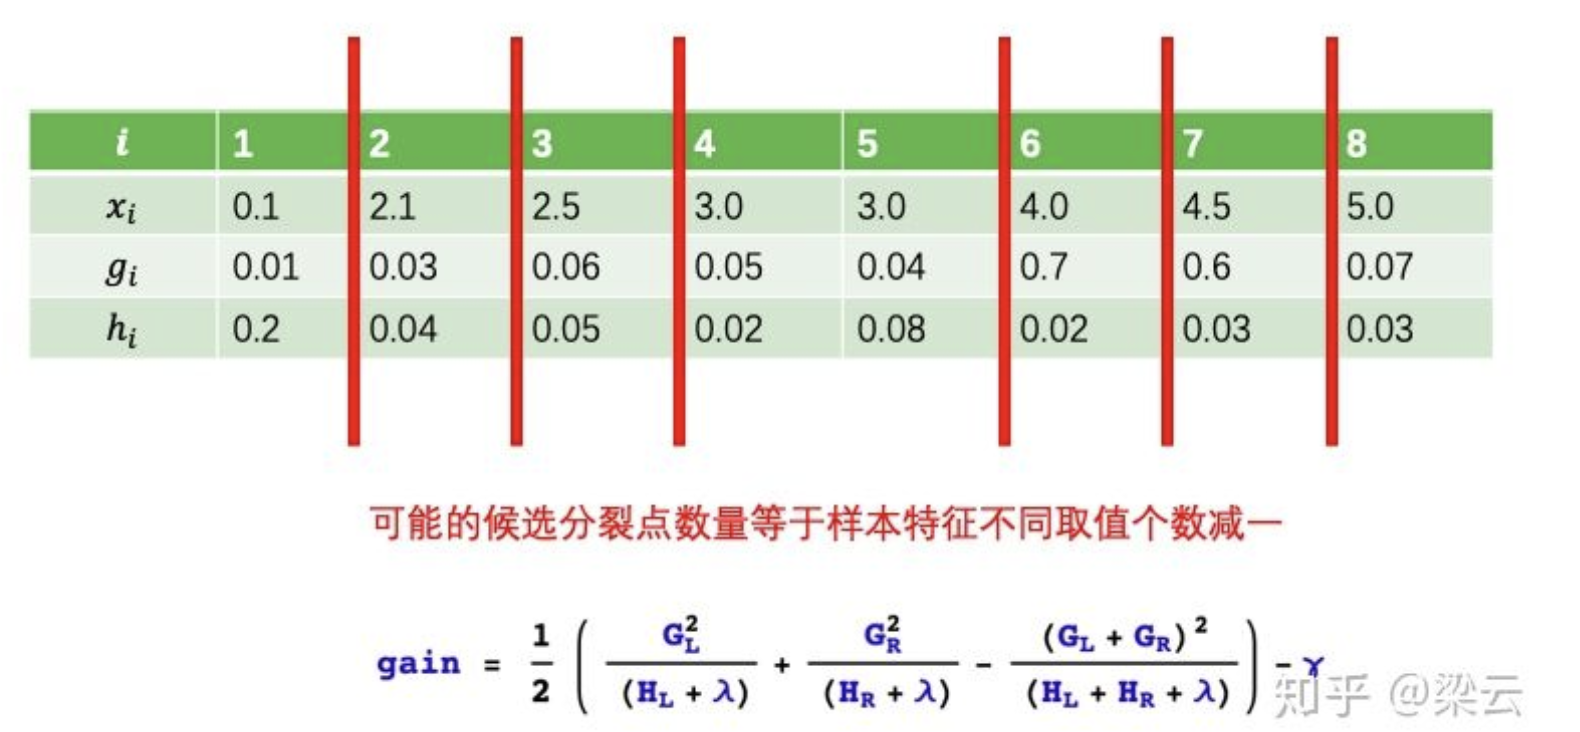
\includegraphics[width=1\textwidth]{fig/LightGBM_PreOrder_Example.png}
\end{figure}

直方图算法如下:
\begin{figure}[H]
    \centering
    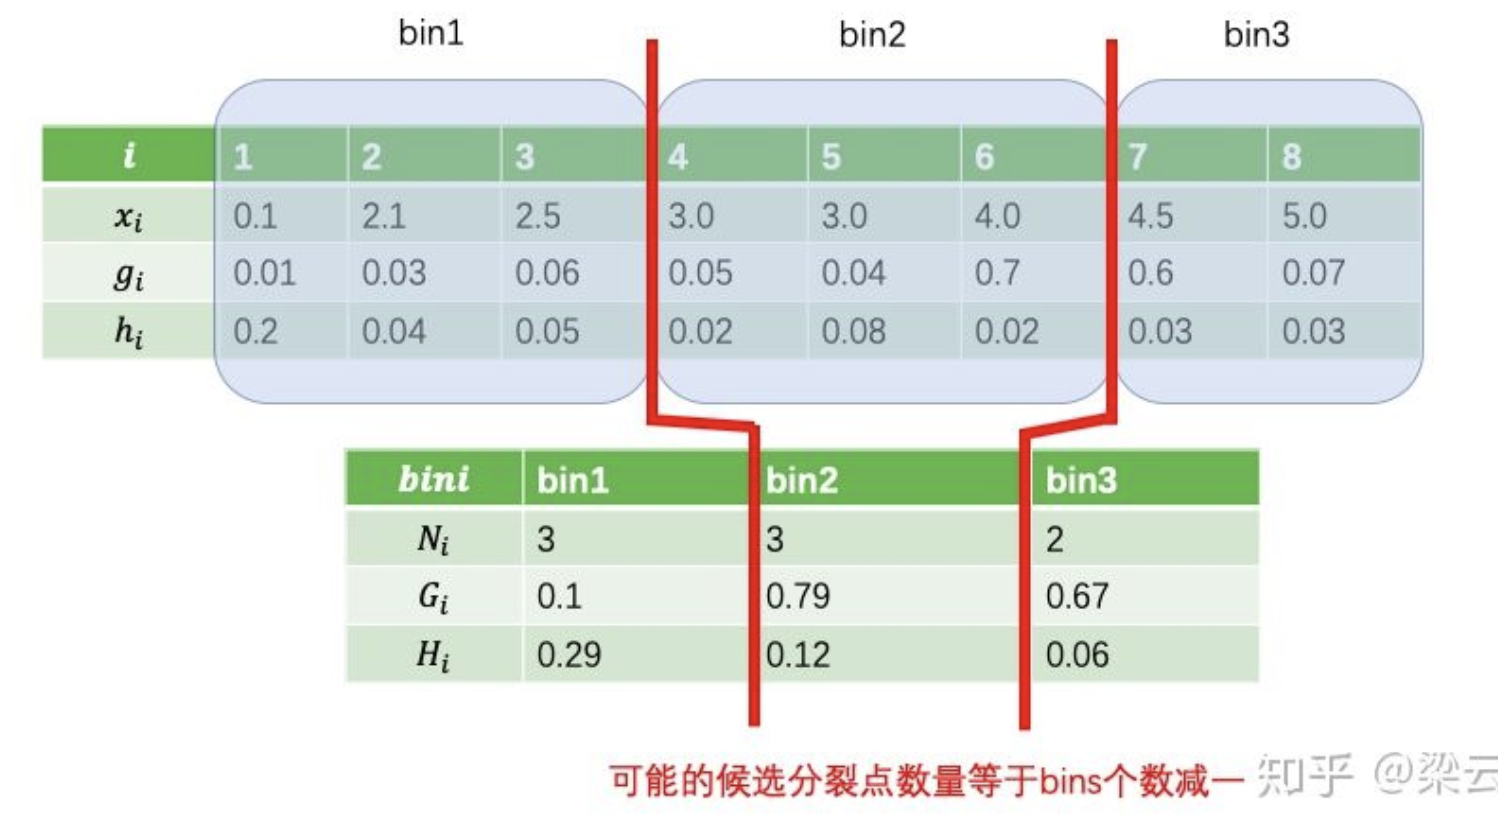
\includegraphics[width=1\textwidth]{fig/LightGBM_Histogram_Example.png}
\end{figure}

直方图差加速如下:
\begin{figure}[H]
    \centering
    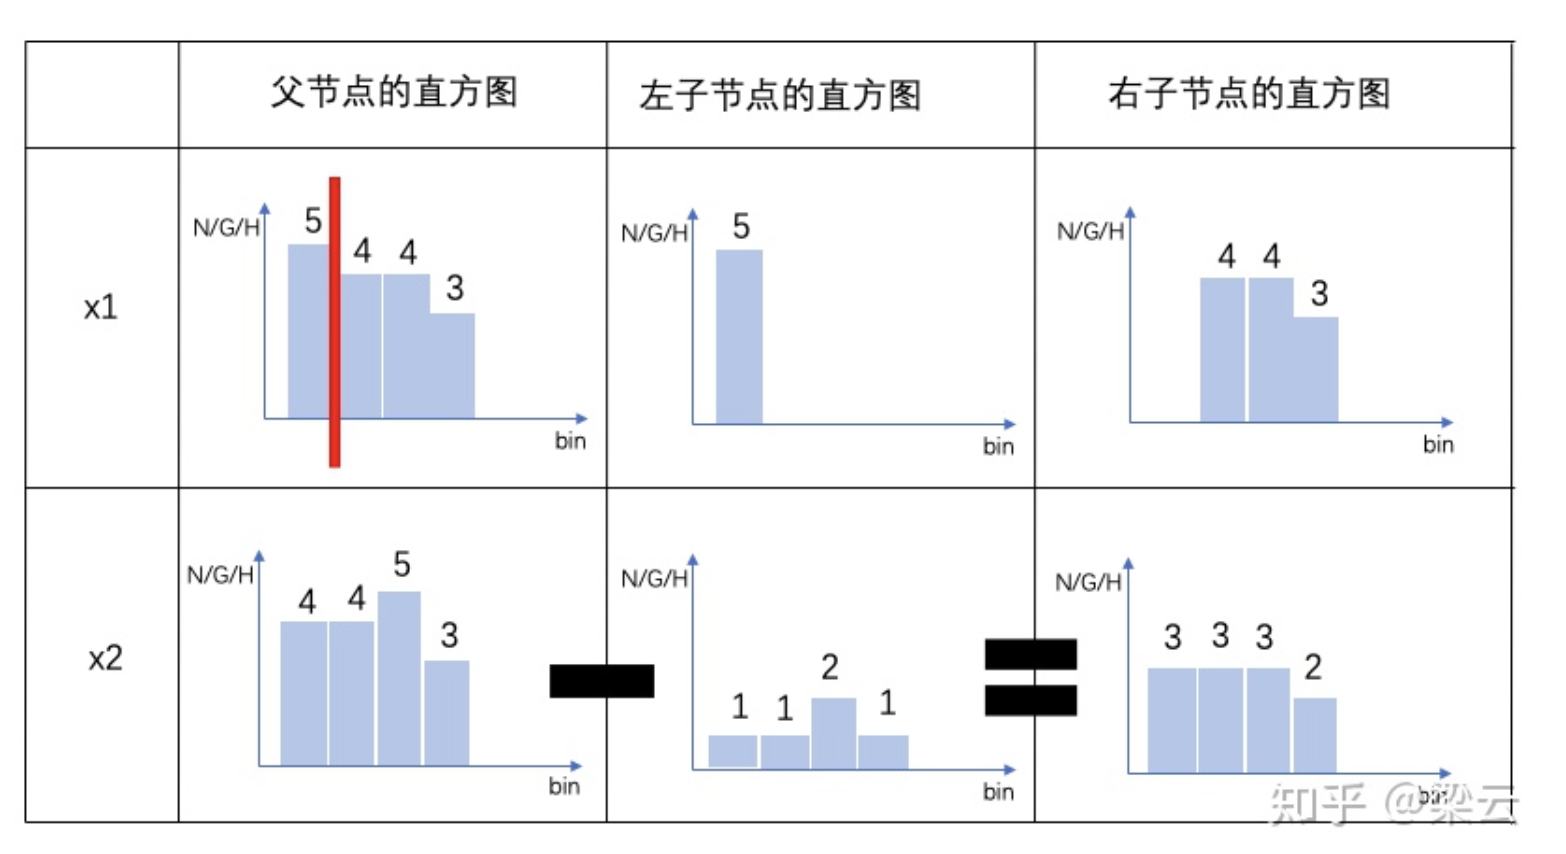
\includegraphics[width=1\textwidth]{fig/LightGBM_Histogram_Diff_Example.png}
\end{figure}

\subsection{GOSS算法}
GOSS算法全称为Gradient-based One-Side Sampling,即基于梯度的单边采样算法。其主要思想是通过对样本采样的方法来减少计算目标函数增益时候的复杂度。

如果对全部样本进行随机采样,势必会对目标函数增益的计算精度造成较大的影响。GOSS算法的创新之处在于它只对梯度绝对值较小的样本按照一定比例进行采样,而保留了梯度绝对值较大的样本。这就是所谓的单边采样。\textbf{由于目标函数增益主要来自于梯度绝对值较大的样本,因此这种方法在计算性能和计算精度之间取得了很好的平衡}。

基于梯度的单边采样算法如下:
\begin{figure}[H]
    \centering
    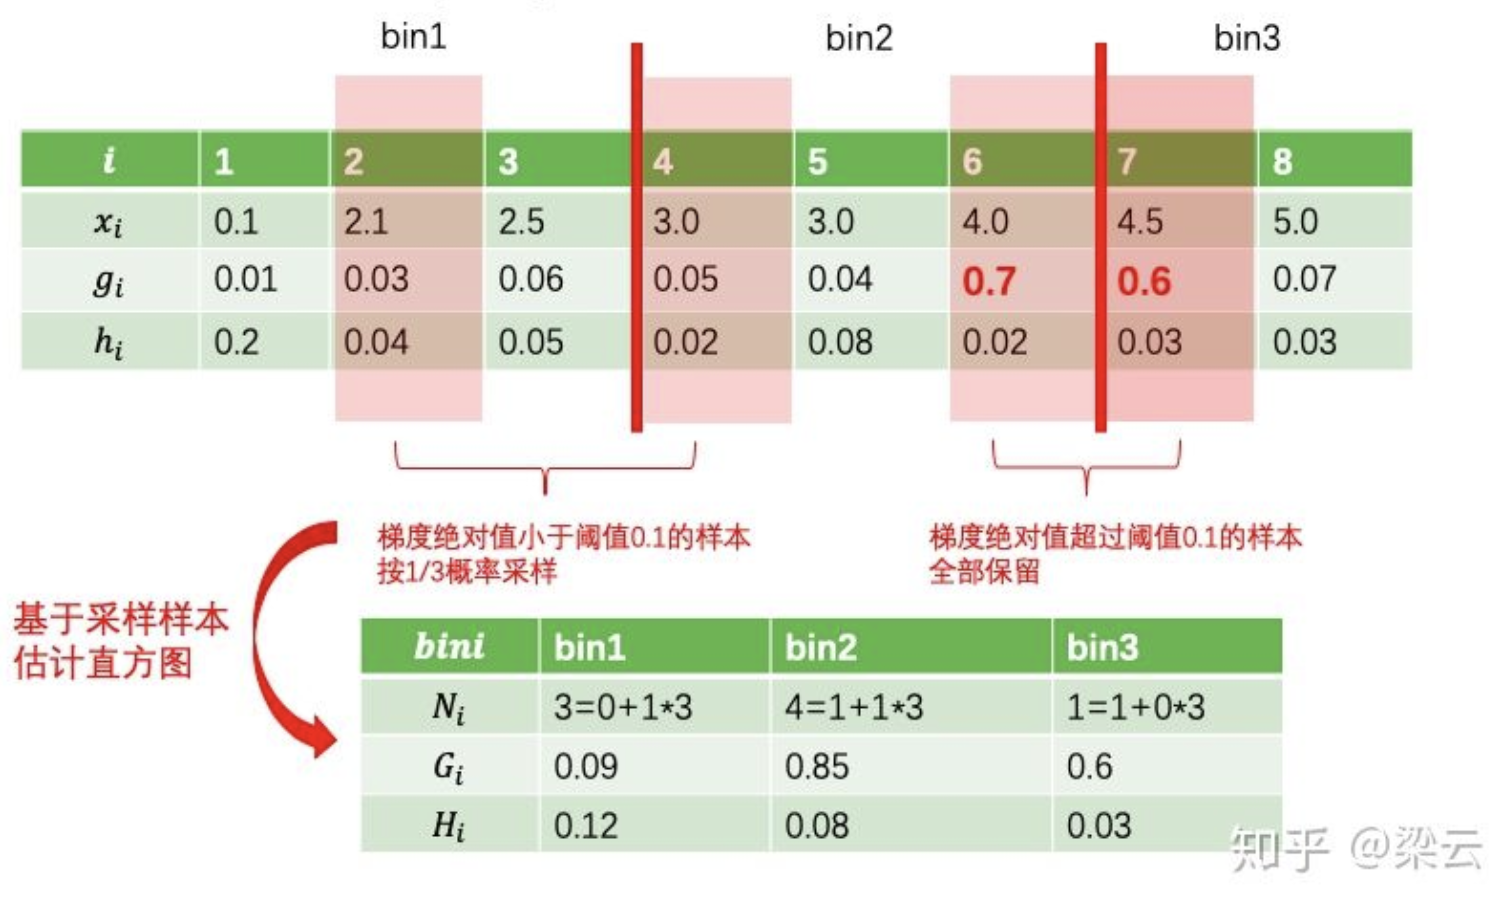
\includegraphics[width=1\textwidth]{fig/LightGBM_GOSS_Example.png}
\end{figure}

\subsection{EFB算法}
EFB算法全称是Exclusive Feature Bundling,即互斥特征绑定算法。

EFB算法可以有效减少用于构建直方图的特征数量,从而降低计算复杂度,尤其是特征中包含大量稀疏特征的时候。

在许多应用场景下,数据集中会有大量的稀疏特征,这些稀疏特征大部分样本都取值为0,只有少数样本取值非0。通常可以认为这些稀疏特征是互斥的,即它们几乎不会同时取非零值。利用这种特性,可以通过对某些特征的取值重新编码,将多个这样互斥的特征捆绑成为一个新的特征。

有趣的是,\textbf{对于类别特征,如果转换成onehot编码,则这些onehot编码后的多个特征相互之间是互斥的,从而可以被捆绑成为一个特征}。因此,对于指定为类别特征的特征,LightGBM可以直接将每个类别取值和一个bin关联,从而自动地处理它们,而无需预处理成onehot编码多此一举。
\begin{figure}[H]
    \centering
    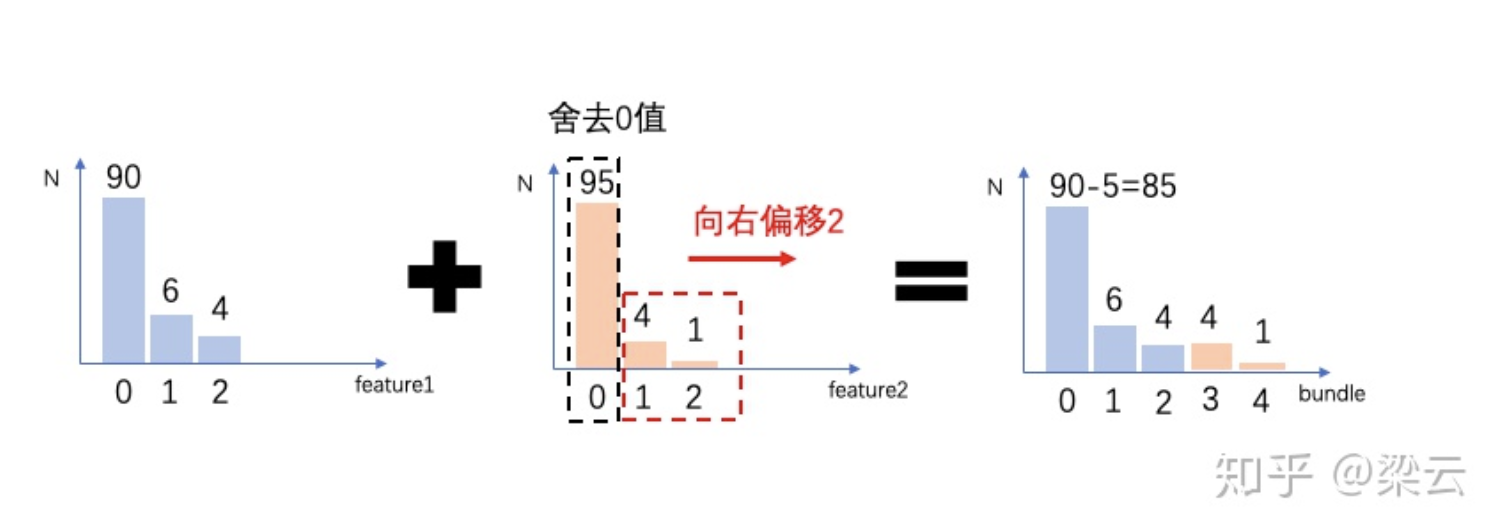
\includegraphics[width=1\textwidth]{fig/LightGBM_EFB_Example.png}
\end{figure}

\begin{framed}
举个例子,对于一列特征[1,nan,1,nan,1]和一列特征[nan,1,nan,1,nan],他们正好可以合并成一列特征[1,2,1,2,1]。LGB的目标就是在于找到这样的特征并且将他们合并在一起。

如果把特征抽象成图中的点,特征之间的冲突看作是图中的边,那么问题就转换为找出图中的社团并使图中的社团数量最少。LGB里提出了一个贪心的策略,按照有权度来为图中所有的点排序,然后把特征合并到度小于某个阈值的社团中或单独创建一个社团。

如果把特征抽象成图中的点,特征之间的冲突看作是图中的边,那么问题就转换为找出图中的社团并使图中的社团数量最少。LGB里提出了一个贪心的策略,按照有权度来为图中所有的点排序,然后把特征合并到度小于某个阈值的社团中或单独创建一个社团。也就是说,该问题可以被转化为图上色问题,并通过贪婪算法求解。

对于特征如何合并,一个重要的原则就是使合并的两个特征可以被顺利区分出来,LGB采取了一个更改阈值的方法。例如对于特征$x \in (0, 10)$, 特征$y \in (0, 20)$,就可以把特征$y$转换为$y \in (10,30)$,然后再去合并$x$与$y$。
\end{framed}

\section{常见问题\cite{XGBoost_20_Common_Questions}}
\subsection{XGBoost 相关问题}
\subsubsection{简单介绍一下XGBoost}
首先需要说一说GBDT,它是一种基于boosting增强策略的加法模型,训练的时候采用前向分布算法进行贪婪的学习,每次迭代都学习一棵CART树来拟合之前 $t-1$ 棵树的预测结果与训练样本真实值的残差。

XGBoost对GBDT进行了一系列优化,比如损失函数进行了二阶泰勒展开、目标函数加入正则项、支持并行和默认缺失值处理等,在可扩展性和训练速度上有了巨大的提升,但其核心思想没有大的变化。


\subsubsection{XGBoost为什么可以并行训练}
XGBoost的并行,并不是说每棵树可以并行训练,XGB本质上仍然采用boosting思想,每棵树训练前需要等前面的树训练完成才能开始训练。

XGBoost的并行,指的是特征维度的并行:在训练之前,每个特征按特征值对样本进行预排序,并存储为Block结构,在后面查找特征分割点时可以重复使用,而且特征已经被存储为一个个block结构,那么在寻找每个特征的最佳分割点时,可以利用多线程对每个block并行计算。

\subsubsection{XGBoost为什么快}
\begin{itemize}
\setlength{\itemsep}{0pt}
\setlength{\parsep}{0pt}
\setlength{\parskip}{0pt}
    \item \textbf{分块并行}:训练前每个特征按特征值进行排序并存储为Block结构,后面查找特征分割点时重复使用,并且支持并行查找每个特征的分割点。
    \item \textbf{候选分位点}:每个特征采用常数个分位点作为候选分割点。
    \item \textbf{CPU cache 命中优化}:使用缓存预取的方法,对每个线程分配一个连续的buffer,读取每个block中样本的梯度信息并存入连续的Buffer中。
    \item \textbf{Block 处理优化}:Block预先放入内存;Block按列进行解压缩;将Block划分到不同硬盘来提高吞吐。
\end{itemize}

\subsubsection{XGBoost防止过拟合的方法}
\begin{itemize}
\setlength{\itemsep}{0pt}
\setlength{\parsep}{0pt}
\setlength{\parskip}{0pt}
    \item \textbf{目标函数添加正则项}:叶子节点个数+叶子节点权重的L2正则化。
    \item \textbf{列抽样}:训练的时候只用一部分特征(不考虑剩余的block块即可)。
    \item \textbf{子采样}:每轮计算可以不使用全部样本,使算法更加保守。
    \item \textbf{shrinkage}:可以叫学习率或步长,为了给后面的训练留出更多的学习空间。
\end{itemize}

\subsubsection{XGBoost如何处理缺失值}
XGBoost模型的一个优点就是允许特征存在缺失值。对缺失值的处理方式如下:
\begin{itemize}
\setlength{\itemsep}{0pt}
\setlength{\parsep}{0pt}
\setlength{\parskip}{0pt}
    \item 在特征k上寻找最佳 split point 时,不会对该列特征 missing 的样本进行遍历,而只对该列特征值为 non-missing 的样本上对应的特征值进行遍历,通过这个技巧来减少了为稀疏离散特征寻找 split point 的时间开销。
    \item 在逻辑实现上,为了保证完备性,会将该特征值missing的样本分别分配到左叶子结点和右叶子结点,两种情形都计算一遍后,选择分裂后增益最大的那个方向(左分支或是右分支),作为预测时特征值缺失样本的默认分支方向。
    \item 如果在训练中没有缺失值而在预测中出现缺失,那么会自动将缺失值的划分方向放到右子结点。
\end{itemize}

\subsubsection{XGBoost中的一棵树的停止生长条件}
当新引入的一次分裂所带来的增益Gain<0时,放弃当前的分裂。这是训练损失和模型结构复杂度的博弈过程。

当树达到最大深度时,停止建树,因为树的深度太深容易出现过拟合,这里需要设置一个超参数max\_depth。

当引入一次分裂后,重新计算新生成的左、右两个叶子结点的样本权重和。如果任一个叶子结点的样本权重低于某一个阈值,也会放弃此次分裂。这涉及到一个超参数:最小样本权重和,是指如果一个叶子节点包含的样本数量太少也会放弃分裂,防止树分的太细。

\subsubsection{XGBoost如何处理不平衡数据}
对于不平衡的数据集,例如用户的购买行为,肯定是极其不平衡的,这对XGBoost的训练有很大的影响,XGBoost有两种自带的方法来解决:

第一种,如果你在意AUC,采用AUC来评估模型的性能,那你可以通过设置scale\_pos\_weight来平衡正样本和负样本的权重。例如,当正负样本比例为1:10时,scale\_pos\_weight可以取10;

第二种,如果你在意概率(预测得分的合理性),你不能重新平衡数据集(会破坏数据的真实分布),应该设置max\_delta\_step为一个有限数字来帮助收敛(基模型为LR时有效)。

那么,源码到底是怎么利用scale\_pos\_weight来平衡样本的呢,是调节权重还是过采样呢?请看源码:
\begin{figure}[H]
    \centering
    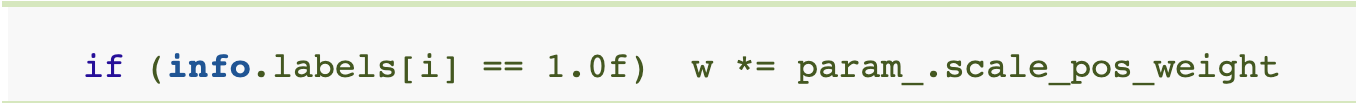
\includegraphics[width=1\textwidth]{fig/XGBoost_Code_Sample_Weight.png}
\end{figure}
可以看出,应该是增大了少数样本的权重。

除此之外,还可以通过上采样、下采样、SMOTE算法或者自定义代价函数的方式解决正负样本不平衡的问题。

\subsubsection{XGBoost中如何对树进行剪枝}
在目标函数中增加了正则项:使用叶子结点的数目和叶子结点权重的$L_2$模的平方,控制树的复杂度。

在结点分裂时,定义了一个阈值,如果分裂后目标函数的增益小于该阈值,则不分裂。

当引入一次分裂后,重新计算新生成的左、右两个叶子结点的样本权重和。如果任一个叶子结点的样本权重低于某一个阈值(最小样本权重和),也会放弃此次分裂。

XGBoost 先从顶到底建立树直到最大深度,再从底到顶反向检查是否有不满足分裂条件的结点,进行剪枝。

\subsubsection{XGBoost如何选择最佳分裂点? }
XGBoost在训练前预先将特征按照特征值进行了排序,并存储为block结构,以后在结点分裂时可以重复使用该结构。

因此,可以采用特征并行的方法利用多个线程分别计算每个特征的最佳分割点,根据每次分裂后产生的增益,最终选择增益最大的那个特征的特征值作为最佳分裂点。

如果在计算每个特征的最佳分割点时,对每个样本都进行遍历,计算复杂度会很大,这种全局扫描的方法并不适用大数据的场景。XGBoost还提供了一种直方图近似算法,对特征排序后仅选择常数个候选分裂位置作为候选分裂点,极大提升了结点分裂时的计算效率。

\subsubsection{XGBoost的Scalable性如何体现}
\textbf{基分类器的scalability}:弱分类器可以支持CART决策树,也可以支持LR和Linear。

\textbf{目标函数的scalability}:支持自定义loss function,只需要其一阶、二阶可导。有这个特性是因为泰勒二阶展开,得到通用的目标函数形式。

\textbf{学习方法的scalability}:Block结构支持并行化,支持 Out-of-core计算。

\subsubsection{XGBoost如何评价特征的重要性}
我们采用三种方法来评判XGBoost模型中特征的重要程度:

\textbf{weight}:该特征在所有树中被用作分割样本的特征的总次数。

\textbf{gain} :该特征在其出现过的所有树中产生的平均增益。

\textbf{cover} :该特征在其出现过的所有树中的平均覆盖范围。覆盖范围这里指的是一个特征用作分割点后,其影响的样本数量,即有多少样本经过该特征分割到两个子节点。

\subsubsection{XGBooost参数调优的一般步骤}
首先需要初始化一些基本变量,例如:
\begin{itemize}
\setlength{\itemsep}{0pt}
\setlength{\parsep}{0pt}
\setlength{\parskip}{0pt}
    \item max\_depth = 5
    \item min\_child\_weight = 1
    \item gamma = 0
    \item subsample, colsample\_bytree = 0.8
    \item scale\_pos\_weight = 1
\end{itemize}

(1) 确定learning rate和estimator的数量

learning rate可以先用0.1,用cv来寻找最优的estimators

(2) max\_depth和 min\_child\_weight
我们调整这两个参数是因为,这两个参数对输出结果的影响很大。我们首先将这两个参数设置为较大的数,然后通过迭代的方式不断修正,缩小范围。

max\_depth,每棵子树的最大深度,check from range(3,10,2)。

min\_child\_weight,子节点的权重阈值,check from range(1,6,2)。

如果一个结点分裂后,它的所有子节点的权重之和都大于该阈值,该叶子节点才可以划分。

(3) gamma

也称作最小划分损失min\_split\_loss,check from 0.1 to 0.5,指的是,对于一个叶子节点,当对它采取划分之后,损失函数的降低值的阈值。

如果大于该阈值,则该叶子节点值得继续划分;如果小于该阈值,则该叶子节点不值得继续划分

(4) subsample, colsample\_bytree

subsample是对训练的采样比例;

colsample\_bytree是对特征的采样比例;

both check from 0.6 to 0.9

(5) 正则化参数

alpha 是$L_1$正则化系数,try 1e-5, 1e-2, 0.1, 1, 100

lambda 是$L_2$正则化系数

(6) 降低学习率

降低学习率的同时增加树的数量,通常最后设置学习率为0.01~0.1


\subsubsection{XGBoost模型如果过拟合了怎么解决}
当出现过拟合时,有两类参数可以缓解:

第一类参数:用于直接控制模型的复杂度。包括max\_depth,min\_child\_weight,  gamma 等参数

第二类参数:用于增加随机性,从而使得模型在训练时对于噪音不敏感。包括subsample,colsample\_bytree

还有就是直接减小learning rate,但需要同时增加estimator 参数。

\subsubsection{为什么XGBoost相比某些模型对缺失值不敏感}
对存在缺失值的特征,一般的解决方法是:

离散型变量:用出现次数最多的特征值填充;

连续型变量:用中位数或均值填充;

一些模型如SVM和KNN,其模型原理中涉及到了对样本距离的度量,如果缺失值处理不当,最终会导致模型预测效果很差。
而树模型对缺失值的敏感度低,大部分时候可以在数据缺失时时使用。原因就是,一棵树中每个结点在分裂时,寻找的是某个特征的最佳分裂点(特征值),完全可以不考虑存在特征值缺失的样本,也就是说,如果某些样本缺失的特征值缺失,对寻找最佳分割点的影响不是很大。
XGBoost对缺失数据有特定的处理方法,
因此,对于有缺失值的数据在经过缺失处理后:
当数据量很小时,优先用朴素贝叶斯;数据量适中或者较大,用树模型,优先XGBoost;数据量较大,也可以用神经网络;避免使用距离度量相关的模型,如KNN和SVM


\subsection{不同模型的比较}
\subsubsection{XGBoost与GBDT有什么不同}
\begin{itemize}
\setlength{\itemsep}{0pt}
\setlength{\parsep}{0pt}
\setlength{\parskip}{0pt}
    \item \textbf{基分类器}:XGBoost的基分类器不仅支持CART决策树,还支持线性分类器,此时XGBoost相当于带L1和L2正则化项的Logistic回归(分类问题)或者线性回归(回归问题)。
    \item \textbf{导数信息}:XGBoost对损失函数做了二阶泰勒展开,GBDT只用了一阶导数信息,并且XGBoost还支持自定义损失函数,只要损失函数一阶、二阶可导。
    \item \textbf{正则项}:XGBoost的目标函数加了正则项,相当于预剪枝,使得学习出来的模型更加不容易过拟合。
    \item \textbf{列抽样}:XGBoost支持列采样,与随机森林类似,用于防止过拟合
    \item \textbf{缺失值处理}:对树中的每个非叶子结点,XGBoost可以自动学习出它的默认分裂方向。如果某个样本该特征值缺失,会将其划入默认分支。
    \item \textbf{并行化}:注意不是tree维度的并行,而是特征维度的并行。XGBoost预先将每个特征按特征值排好序,存储为块结构,分裂结点时可以采用多线程并行查找每个特征的最佳分割点,极大提升训练速度
\end{itemize}

\subsubsection{RF和GBDT的区别}
相同点:
\begin{itemize}
\setlength{\itemsep}{0pt}
\setlength{\parsep}{0pt}
\setlength{\parskip}{0pt}
    \item 都是由多棵树组成,最终的结果都是由多棵树一起决定。
\end{itemize}

不同点:
\begin{itemize}
\setlength{\itemsep}{0pt}
\setlength{\parsep}{0pt}
\setlength{\parskip}{0pt}
    \item 集成学习:RF属于bagging思想,而GBDT是boosting思想。
    \item 偏差-方差权衡:RF不断的降低模型的方差,而GBDT不断的降低模型的偏差。
    \item 训练样本:RF每次迭代的样本是从全部训练集中有放回抽样形成的,而GBDT每次使用全部样本
    \item 并行性:RF的树可以并行生成,而GBDT只能顺序生成(需要等上一棵树完全生成)
    \item 最终结果:RF最终是多棵树进行多数表决(回归问题是取平均),而GBDT是加权融合
    \item 数据敏感性:RF对异常值不敏感,而GBDT对异常值比较敏感
    \item 泛化能力:RF不易过拟合,而GBDT容易过拟合
\end{itemize}

\subsubsection{比较LR和GBDT,说说什么情景下GBDT不如LR}
先说说LR和GBDT的区别:
\begin{itemize}
\setlength{\itemsep}{0pt}
\setlength{\parsep}{0pt}
\setlength{\parskip}{0pt}
    \item LR是线性模型,可解释性强,很容易并行化,但学习能力有限,需要大量的人工特征工程;
    \item GBDT是非线性模型,具有天然的特征组合优势,特征表达能力强,但是树与树之间无法并行训练,而且树模型很容易过拟合;
\end{itemize}

当在高维稀疏特征的场景下,LR的效果一般会比GBDT好。原因如下:

先看一个例子:假设一个二分类问题,label为0和1,特征有100维,如果有1w个样本,但其中只要10个正样本1,而这些样本的特征 $f_1$的值为全为1,而其余9990条样本的$f_1$特征都为0(在高维稀疏的情况下这种情况很常见)。

我们都知道在这种情况下,树模型很容易优化出一个使用$f_1$特征作为重要分裂节点的树,因为这个结点直接能够将训练数据划分的很好,但是当测试的时候,却会发现效果很差,因为这个特征$f_1$只是刚好偶然间跟$y$拟合到了这个规律,这也是我们常说的过拟合。

那么这种情况下,如果采用LR的话,应该也会出现类似过拟合的情况呀:$y = W_1*f_1 + \cdots + W_i*f_i + + ….$,其中 $W_1$特别大以拟合这10个样本。为什么此时树模型就过拟合的更严重呢?

仔细想想发现,因为现在的模型普遍都会带着正则项,而 LR 等线性模型的正则项是对权重的惩罚,也就是 $W_1$一旦过大,惩罚就会很大,进一步压缩 $W_1 $的值,使他不至于过大。但是,树模型则不一样,\textbf{树模型的惩罚项通常为叶子节点数和深度等},而我们都知道,对于上面这种 case,树只需要一个节点就可以完美分割9990和10个样本,一个结点,最终产生的惩罚项极其之小。

这也就是为什么在高维稀疏特征的时候,线性模型会比非线性模型好的原因了:\textbf{带正则化的线性模型比较不容易对稀疏特征过拟合}。

\subsubsection{XGBoost和LightGBM的区别}
\textbf{(1)树生长策略}:XGB采用level-wise的分裂策略,LGB采用leaf-wise的分裂策略。XGB对每一层所有节点做无差别分裂,但是可能有些节点增益非常小,对结果影响不大,带来不必要的开销。Leaf-wise是在所有叶子节点中选取分裂收益最大的节点进行的,但是很容易出现过拟合问题,所以需要对最大深度做限制。
\begin{figure}[H]
    \centering
    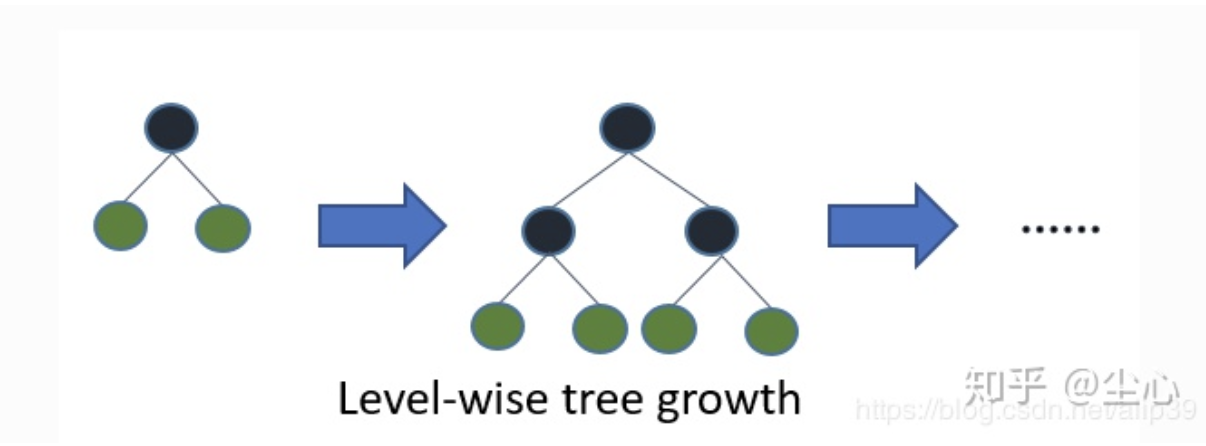
\includegraphics[width=.6\textwidth]{fig/LightGBM_Node_Split_Level_Wise.png}
\end{figure}
\begin{figure}[H]
    \centering
    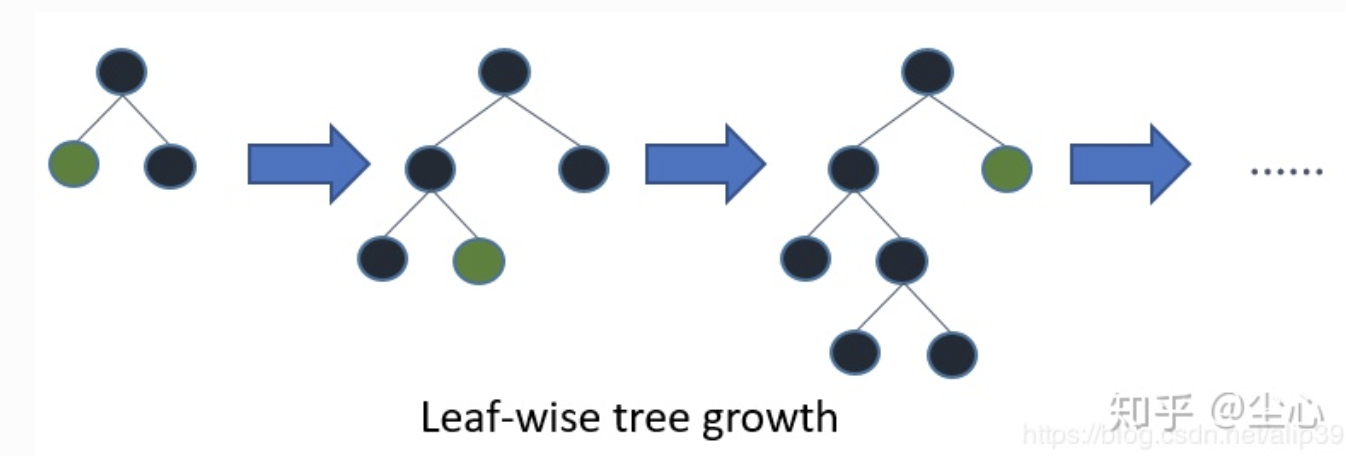
\includegraphics[width=.6\textwidth]{fig/LightGBM_Node_Split_Leaf_Wise.png}
\end{figure}

Level-wise过一次数据可以同时分裂同一层的叶子,容易进行多线程优化,也好控制模型复杂度,不容易过拟合。但实际上Level-wise是一种低效的算法,因为它不加区分的对待同一层的叶子,带来了很多没必要的开销,因为实际上很多叶子的分裂增益较低,没必要进行搜索和分裂。

在Histogram算法之上,LightGBM进行进一步的优化,采用的Leaf-wise则是一种更为高效的策略,每次从当前所有叶子中,找到分裂增益最大的一个叶子,然后分裂,如此循环。

因此同Level-wise相比,在分裂次数相同的情况下,Leaf-wise可以降低更多的误差,得到更好的精度。Leaf-wise的缺点是可能会长出比较深的决策树,产生过拟合。因此LightGBM在Leaf-wise之上增加了一个最大深度的限制,在保证高效率的同时防止过拟合


\textbf{(2)分割点查找算法}:XGB使用特征预排序算法,LGB使用基于直方图的切分点算法,其优势如下:
\begin{itemize}
\setlength{\itemsep}{0pt}
\setlength{\parsep}{0pt}
\setlength{\parskip}{0pt}
    \item 减少内存占用,比如离散为256个bin时,只需要用8位整形就可以保存一个样本被映射为哪个bin(这个bin可以说就是转换后的特征),对比预排序的exact greedy算法来说(用int\_32来存储索引+ 用float\_32保存特征值),可以节省7/8的空间。
;
    \item 计算效率提高,预排序的Exact greedy对每个特征都需要遍历一遍数据,并计算增益,复杂度为O(\#feature$\times$\#data)。而直方图算法在建立完直方图后,只需要对每个特征遍历直方图即可,复杂度为O(\#feature$\times$\#bins)
    \item LGB还可以使用直方图做差加速,一个节点的直方图可以通过父节点的直方图减去兄弟节点的直方图得到,从而加速计算。
\end{itemize}

\begin{framed}
但实际上xgboost的近似直方图算法也类似于lightgbm这里的直方图算法,为什么xgboost的近似算法比lightgbm还是慢很多呢?

xgboost在每一层都动态构建直方图, 因为xgboost的直方图算法不是针对某个特定的feature,而是所有feature共享一个直方图(每个样本的权重是二阶导),所以每一层都要重新构建直方图,而lightgbm中对每个特征都有一个直方图,所以构建一次直方图就够了。
\end{framed}

\textbf{(3)支持离散变量}:无法直接输入类别型变量,因此需要事先对类别型变量进行编码(例如独热编码),而LightGBM可以直接处理类别型变量。

\textbf{(4)缓存命中率}:XGB使用Block结构的一个缺点是取梯度的时候,是通过索引来获取的,而这些梯度的获取顺序是按照特征的大小顺序的,这将导致非连续的内存访问,可能使得CPU cache缓存命中率低,从而影响算法效率。而LGB是基于直方图分裂特征的,梯度信息都存储在一个个bin中,所以访问梯度是连续的,缓存命中率高。

\textbf{(5)LightGBM 与 XGboost 的并行策略不同}:
\begin{itemize}
\setlength{\itemsep}{0pt}
\setlength{\parsep}{0pt}
\setlength{\parskip}{0pt}
    \item \textbf{特征并行} :LGB特征并行的前提是每个worker留有一份完整的数据集,但是每个worker仅在特征子集上进行最佳切分点的寻找;worker之间需要相互通信,通过比对损失来确定最佳切分点;然后将这个最佳切分点的位置进行全局广播,每个worker进行切分即可。XGB的特征并行与LGB的最大不同在于XGB每个worker节点中仅有部分的列数据,也就是垂直切分,每个worker寻找局部最佳切分点,worker之间相互通信,然后在具有最佳切分点的worker上进行节点分裂,再由这个节点广播一下被切分到左右节点的样本索引号,其他worker才能开始分裂。二者的区别就导致了LGB中worker间通信成本明显降低,只需通信一个特征分裂点即可,而XGB中要广播样本索引。
    
    \item \textbf{数据并行 }:当数据量很大,特征相对较少时,可采用数据并行策略。LGB中先对数据水平切分,每个worker上的数据先建立起局部的直方图,然后合并成全局的直方图,采用直方图相减的方式,先计算样本量少的节点的样本索引,然后直接相减得到另一子节点的样本索引,这个直方图算法使得worker间的通信成本降低一倍,因为只用通信以此样本量少的节点。XGB中的数据并行也是水平切分,然后单个worker建立局部直方图,再合并为全局,不同在于根据全局直方图进行各个worker上的节点分裂时会单独计算子节点的样本索引,因此效率贼慢,每个worker间的通信量也就变得很大。
    
    \item \textbf{投票并行(LGB)}:当数据量和维度都很大时,选用投票并行,该方法是数据并行的一个改进。数据并行中的合并直方图的代价相对较大,尤其是当特征维度很大时。大致思想是:每个worker首先会找到本地的一些优秀的特征,然后进行全局投票,根据投票结果,选择top的特征进行直方图的合并,再寻求全局的最优分割点。
\end{itemize}




%\printbibliography
\bibliography{../ref}
\bibliographystyle{IEEEtran}
\end{document}
